\chapter{Grasp Stability Prediction}
\label{cha:tactile}

\begin{chapterabstract}
    \lipsum[2]
\end{chapterabstract}

\clearpage

\section{Introduction}
\label{cha:tactile:sec:introduction}

\begin{figure}[!b]
	\centering
	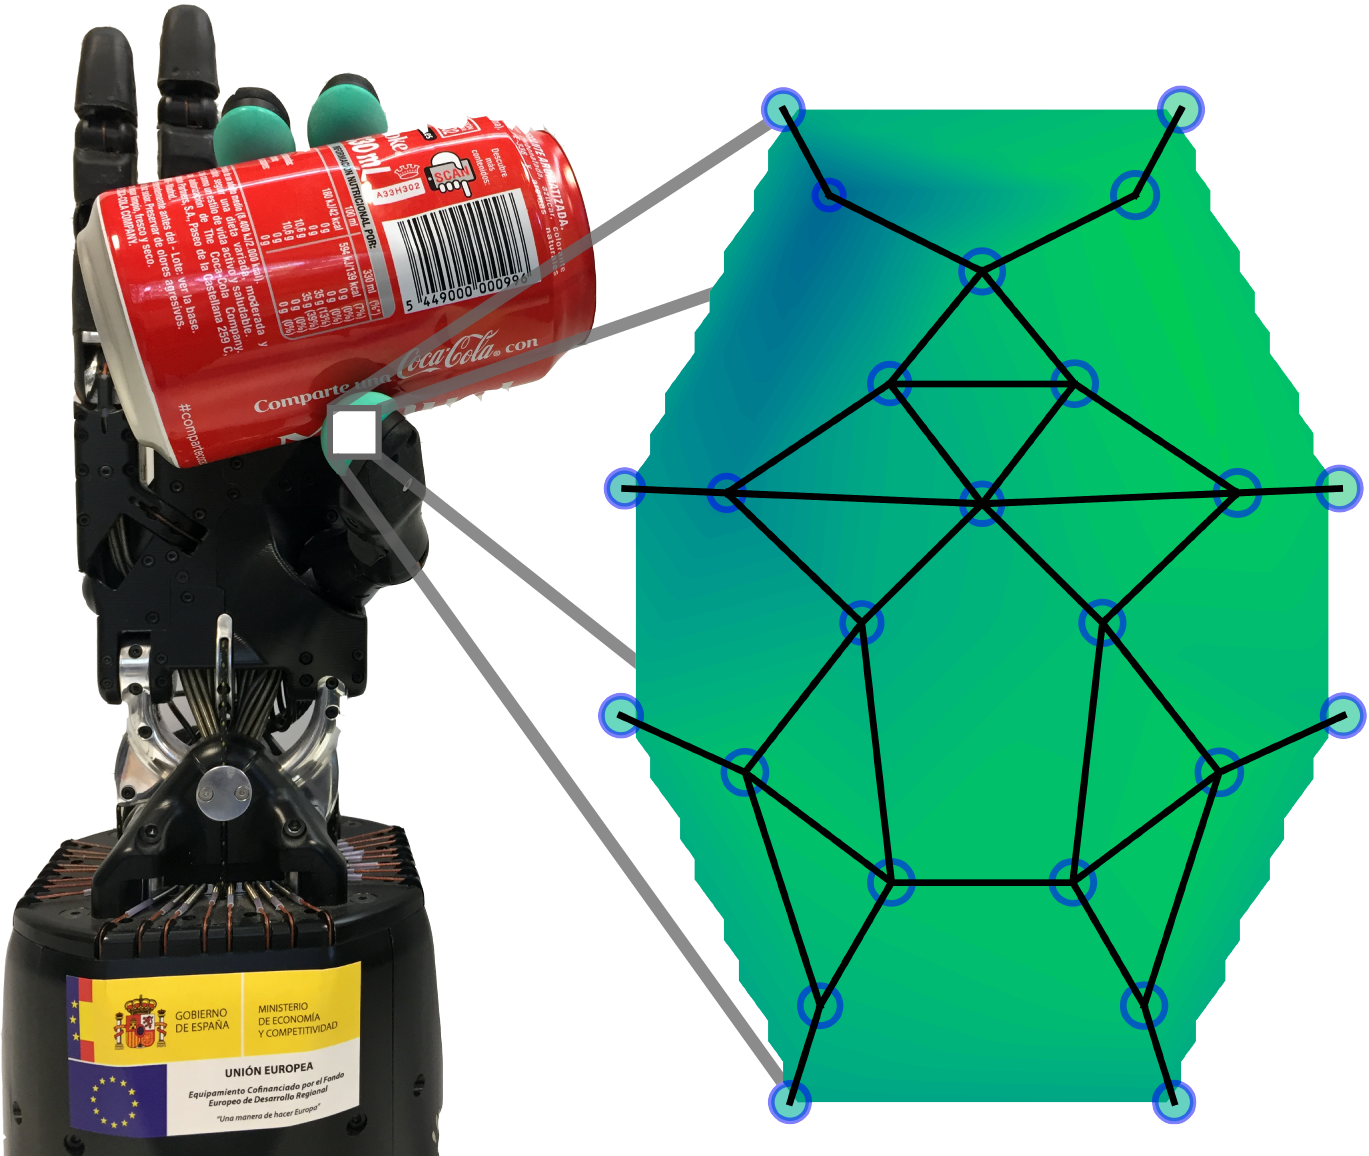
\includegraphics[width = 0.64\textwidth, clip = false, trim = 0 0 0 0]{Figures/Tactile/hand-coke.png}
	\caption{In our proposed TactileGCN framework, we use a Shadow Dexterous hand equipped with three BioTacSP tactile sensors whose readings are transformed into graph representations. Those graphs are then fed as input to a \ac{GCN} in order to learn to predict grasp stability. Figure created by Brayan S. Zapata-Impata and included with his permission.}
	\label{fig:shadow-coke}
\end{figure}

When we humans grasp objects, we intuitively know whether the grip is stable or not even before lifting or manipulating the object. It is not necessary for us to raise our hands or apply any force (either direct such as hitting the object or either indirect such as gravity) in order to determine the object will remain stable between our fingers or our palms. By leveraging our tactile sense, along with our vision and all our intuition and years of experience, we can accurately predict the stability of the grasp for a variety of objects in a wide range of situations. This skill is desirable for any robotic manipulator since it favors the early detection of grasp failures so the robot can react as quick as possible. For instance, a restocking robot working in a store would recognize when an object could slip from its hand and react accordingly and swiftly to avoid a situation in which the object would fall and possibly break down. However easy this task is for a human being, it is not anywhere near as obvious for a robot: there are simply too many variables to take into account for a straightforward solution, e.g., the object's weight, roughness, and geometry; the force of gravity; and the momentum that the object may if we move it to name a few.

The problem of predicting the stability of a grasp is a challenging and ongoing research topic in the field of robotics. The vast majority of the literature, which will be reviewed in depth later in this chapter, makes use of tactile sensors as the main source of data since they provide valuable and abundant information (e.g., temperature or pressure) about the forces that act during the interaction of the robotic hand with the objects \cite{Kappassov2015}. Although methods, datasets, and sensors vary across existing works, all of them agree to distinguish two different states for the grasp: stable, meaning that the object is firmly grasped; or slippery, which means that the object could slide from the hand.

Previous works found in the literature approach this problem following the next methodology: grasp the object, read the tactile sensors equipped in the fingers and/or palm of the hand, calculate custom features that try to characterize these two stability states and learn them in order to make future predictions \cite{Li2014b,Dang2014,Su2015b,Veiga2015}. These proposals treat the tactile readings as classic signals: they preprocess them as if they were arrays, calculate features and learn their characteristics using probabilistic methods. As a consequence, their performance highly depends on the selected characteristics. Moreover, the spatial distribution inherent to the tactile sensor is lost due to the fact of squeezing the data into a one dimensional array.

In this chapter, we propose the use of \acp{GNN} for predicting grasp stability. Since these are deep learning models, there is no need to hand-engineer features because the algorithm is designed for learning them by itself. Moreover, graphs can reflect more accurately the real distribution of the electrodes in the sensor as well as their spatial relationships, which should be of great value for learning tactile features. The main contributions of this chapter can be summarized as follows:

\begin{itemize}
	\item We process tactile readings using a novel perspective: instead of considering them as 1D arrays or 2D images, we build a 3D graph connecting the multiple sensing points (taxels) of the tactile sensor.

	\item We introduce a novel way of processing such information using \acfp{GNN}.
	
	\item We quantitatively check the performance of this new methodology in the real world using a set of tactile sensors installed in a robotic hand.

	\item We release an extension that effectively doubles the size of an already existing dataset \cite{Zapata2018} for grasp stability prediction and includes a whole new split for testing.
\end{itemize}

\clearpage

\section{Background}

In order for the reader to properly understand the following information, we provide brief descriptions of two of the most important concepts introduced in this chapter: tactile sensors and \aclp{GNN}. We suggest the well-versed reader to skip the upcoming sections and move on directly onto the literature review in Section \ref{cha:tactile:sec:relatedworks}.

\subsection{Tactile Sensors}

A tactile sensor is a device which is able to measure information that arises from the phyisical interaction with the environment. Most of this kind of sensors are usually modeled or at least loosely inspired by the biological sense of touch: the cutaneous receptors found in the dermis or epidermis which are able to detect stimuli from pain (nociceptors), chemical substances (chemoreceptors), temperature (thermoreceptors), and mechanical stimulation (mechanoreceptors). From all those kind of receptors, mechanoreceptors and thermoreceptors are the most common in artificial tactile sensors used in robotics and computer hardware. Thanks to those receptors, robots can complement vision systems by leveraging additional information received when the object is being grasped. Although the progress made in learning algorithms can certainly lead to robots being able to predict mechanical properties of the objects, e.g., weight, texture, or stiffness, using vision alone, it is not an effective approach for the time being. However, by taking advantage of tactile sensing when interacting with the object, all those properties can be determined with higher success rates.

Tactile sensors for robotics come in different shapes and sizes featuring a wide range of technologies which includes elastoresistive, capacitive, piezoresistive, and even piezoelectric sensors \cite{Dahiya2012}. Arguably, the most common kind of tactile sensors for robotics are the pressure sensor arrays.

Pressure sensor arrays consist of a grid of tactile elements, also known as \emph{tactels}, each one of them being able of providing pressure or force information when objects contact with them or with the sensor at large. One of the most representative examples of such kind of arrays is the BioTac: a finger-like biomimetic tactile sensor which consist of an array of $19$ impedance sensing electrodes in a rigid core that is immersed in an incompressible and conductive liquid which is in turn surrounded by an elastic skin. It works by detecting the impedance changes on the surface of the rigid core as a result of displacements in the liquid when grasping an object (see Figure \ref{fig:tactile:biotac_sensor}).

\begin{figure}[!thb]
    \centering
    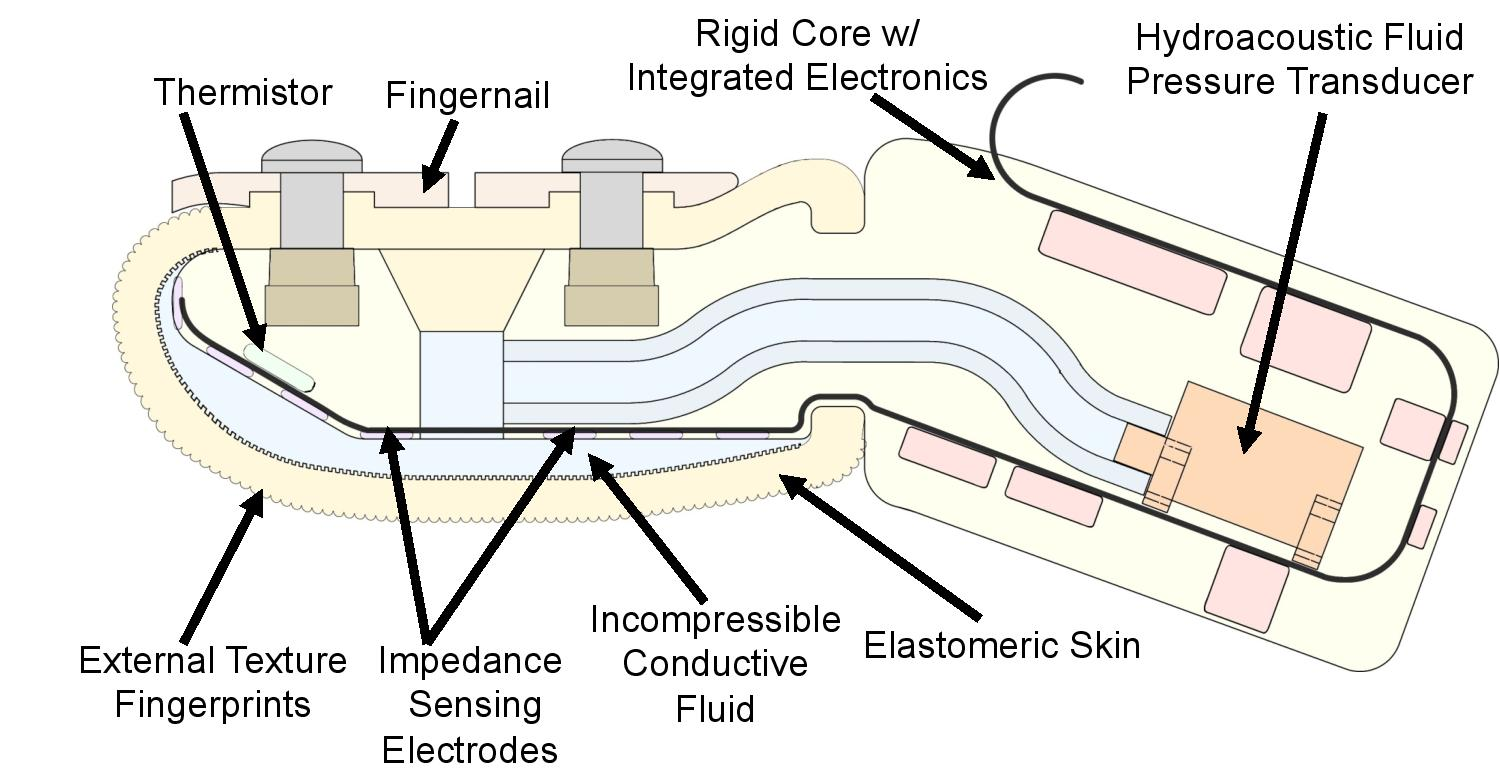
\includegraphics[width=0.65\linewidth]{Figures/Tactile/biotac_1}
    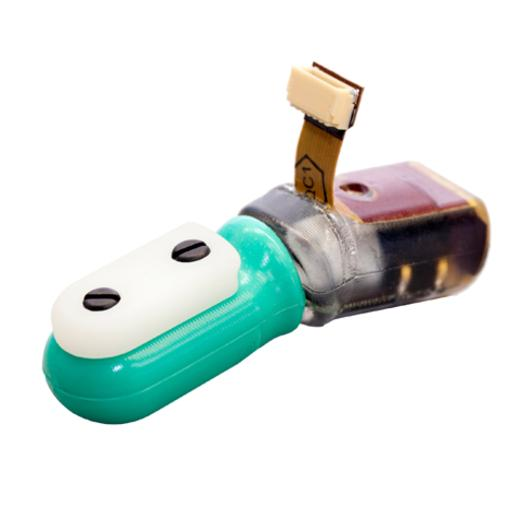
\includegraphics[width=0.34\linewidth]{Figures/Tactile/biotac_2}
    \caption{Cross-section of a BioTac sensor \cite{Syntouch2018} and the actual finger-like product. We can observe how the array of impedance sensing electrodes or tactels are housed in a rigid core which integrates a hydrocoustid fluid pressure transducer as well as a thermistor. The whole package is surrounded by an external and elastomeric skin with external texture fingerprints. The incompressible conductive field is located between the skin and the tactels in the rigid core.}
    \label{fig:tactile:biotac_sensor}
\end{figure}

It is important to remark that the BioTac sensor is also able to provide temperature and heat flow information thanks to a thermistor on the surface of the rigid core that houses the tactels.

In this work, we will make use of a more advanced version of the BioTac sensor which will introduced later in the document for the sake of keeping the background information reduced to the most basic concepts.

\subsection{Graph Neural Networks}

Graph data has been an extremely useful representation for such domains in which it is important not only to define features for the elements themselves but also to provide rich information about the connections that relate them. Some of the domains that can take advante of such kind of data are: document analysis, protein folding, physics systems modeling, and social networks to name a few. Usually the tasks that are carried out when analyzing or learning on graphs are node classification or regression, link prediction, and clustering \cite{Zhou2018}. Lately, graph analysis has achieved even more impact not only due to the aforementioned applications but also to the reformulation of data that traditionally belonged to other domains, e.g., natural language processing or image understanding, as graph-like structures. Most of those cases take advantage of the fact that graph representations are able to properly capture non-Euclidean domains. Figure \ref{fig:tactile:graph_applications} shows examples of various graph representations for different domains.

\begin{figure}[!thb]
    \centering
    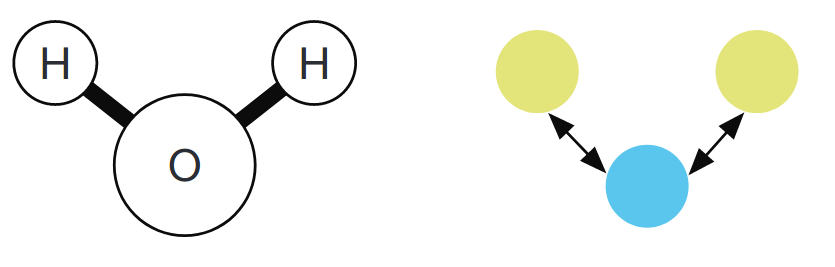
\includegraphics[width=0.49\linewidth]{Figures/Tactile/molecule.png}
    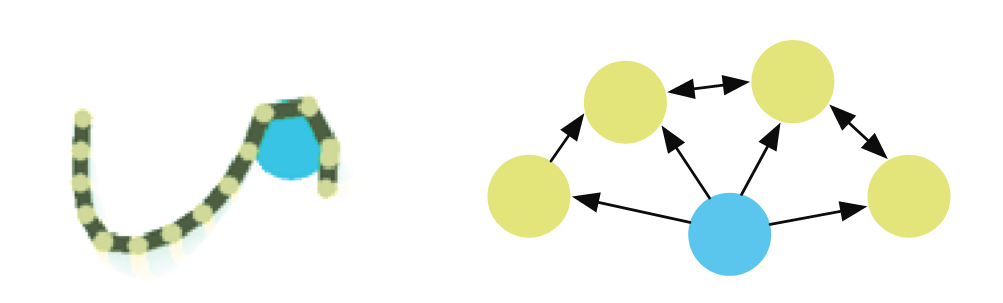
\includegraphics[width=0.49\linewidth]{Figures/Tactile/mass-spring.png}
    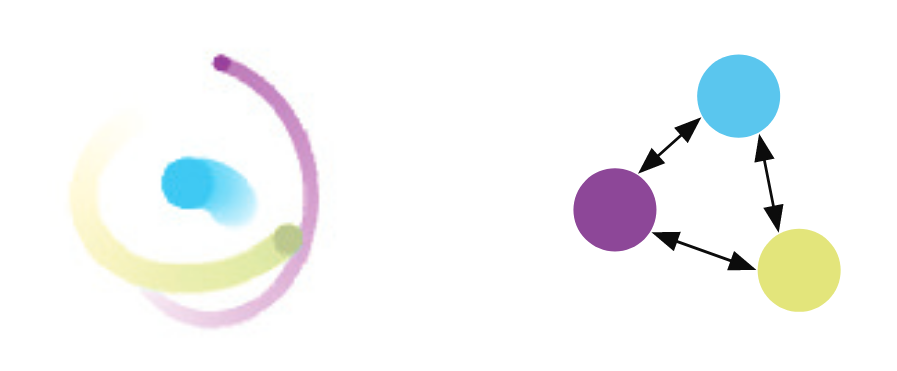
\includegraphics[width=0.49\linewidth]{Figures/Tactile/n-body.png}
    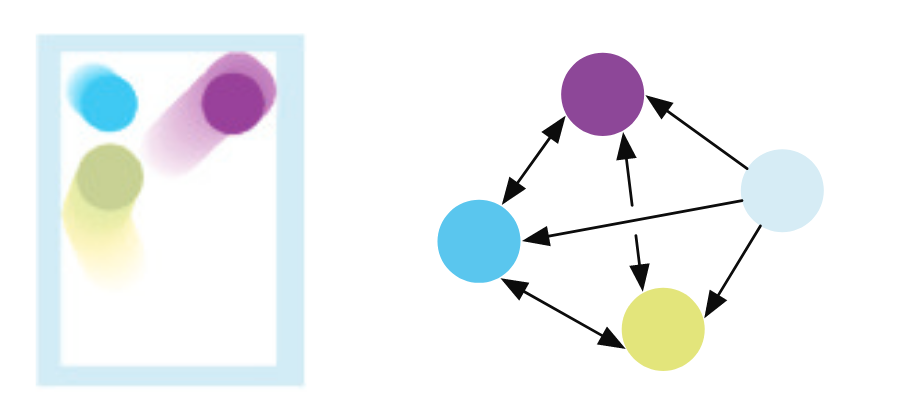
\includegraphics[width=0.49\linewidth]{Figures/Tactile/rigid-body.png}
    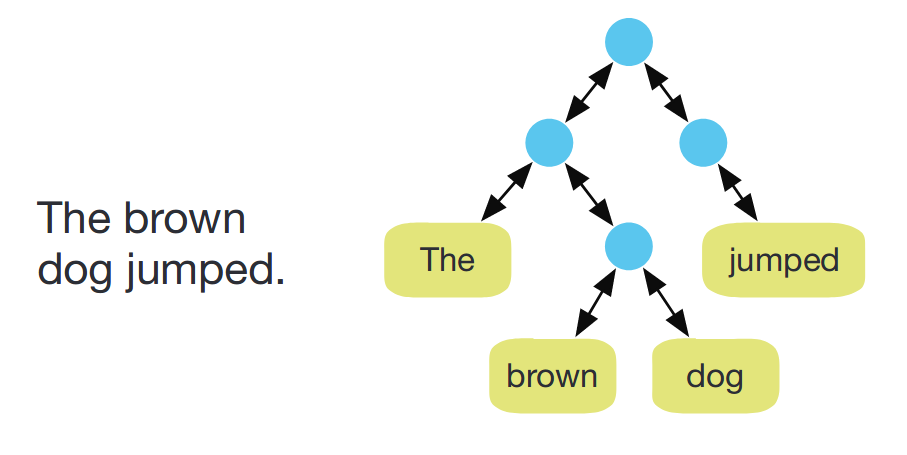
\includegraphics[width=0.49\linewidth]{Figures/Tactile/sentence.png}
    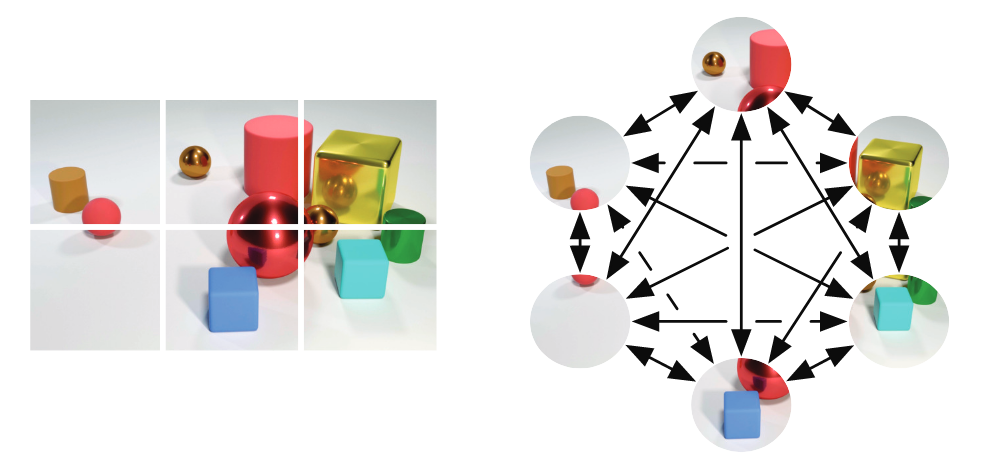
\includegraphics[width=0.49\linewidth]{Figures/Tactile/scene.png}
    \caption{Different graph representations for non-Euclidean domains: a molecule in which each atom is a node and each bond is an edge, a mass-spring system in which the rope is defined by a sequence of masses represented as nodes in the graph, an $n$-body system in which the nodes are the bodies, a rigid-body system, a sentence which can be decomposed into a tree with words as leaves, and a scene-graph which represents a partitioned image and its connections. Figure extracted from \cite{Battaglia2018}.}
    \label{fig:tactile:graph_applications}
\end{figure}

However, despite the usefulnes of graph representations, common and successful architectures such as \aclp{CNN} are not able to deal with non-Euclidean data. As a matter of fact, \acp{CNN} are only able to operate on regular and structured Euclidean representations such as images (\acs{2D} grids) or voxel grids (\acs{3D} grids). Therefore, it is not straightforward to generalize other fruitful architectures such as the \ac{CNN} to graphs mainly due to two reasons: it is hard to define localized filters and pooling operations are not trivial \cite{Zhou2018}.

\acfp{GNN} aim to bridge this gap: they are deep learning architectures which are able to operate directly on non-Euclidean graph domains. The foundations of \acp{GNN} were introduced by Scarselli \emph{et al.} \cite{Scarselli2008} as an extension of traditional neural networks for processing graph data. In this chapter, we will focus on a particular \ac{GNN} architecture that extends the traditional \ac{CNN} one to support operations on graph data: the \acf{GCN}. More details about this architecture will be provided later.

\section{Literature Review}
\label{cha:tactile:sec:relatedworks}

In this section, we review the state of the art of the three main pillars of our work: firstly, we describe previous approaches for predicting grasp stability; secondly, we go through existing datasets which can be used for training grasp stability prediction systems; at last, we explain the most recent and relevant advances in neural networks for graph processing.

\subsection{Grasp Stability Prediction}
\label{cha:tactile:sec:relatedworks:subsec:grasp-stability-prediction}

In the last years, deep learning models have been successfully applied to the problem of grasp stability prediction using tactile sensors as input.

One of the first approaches was taken by Meier \emph{et al.} \cite{Meier2016a}. In this work, they used two piezo-resistive tactile sensor arrays (see Figure \ref{fig:tactile:meier2016}) whose readings were processed to calculate short-time Fourier transforms over a certain window size for each tactel. In this way, they generate spatially arranged stacks of Fourier coefficients to integrate spatial and temporal information in an image-like representation with multiple channels. Then, a \ac{CNN} trained with these matrices is used to predict grasp stability for a dataset of three objects. Furthermore, they also discriminate between rotational and translational slippage.

\begin{figure}[!htb]
    \centering
    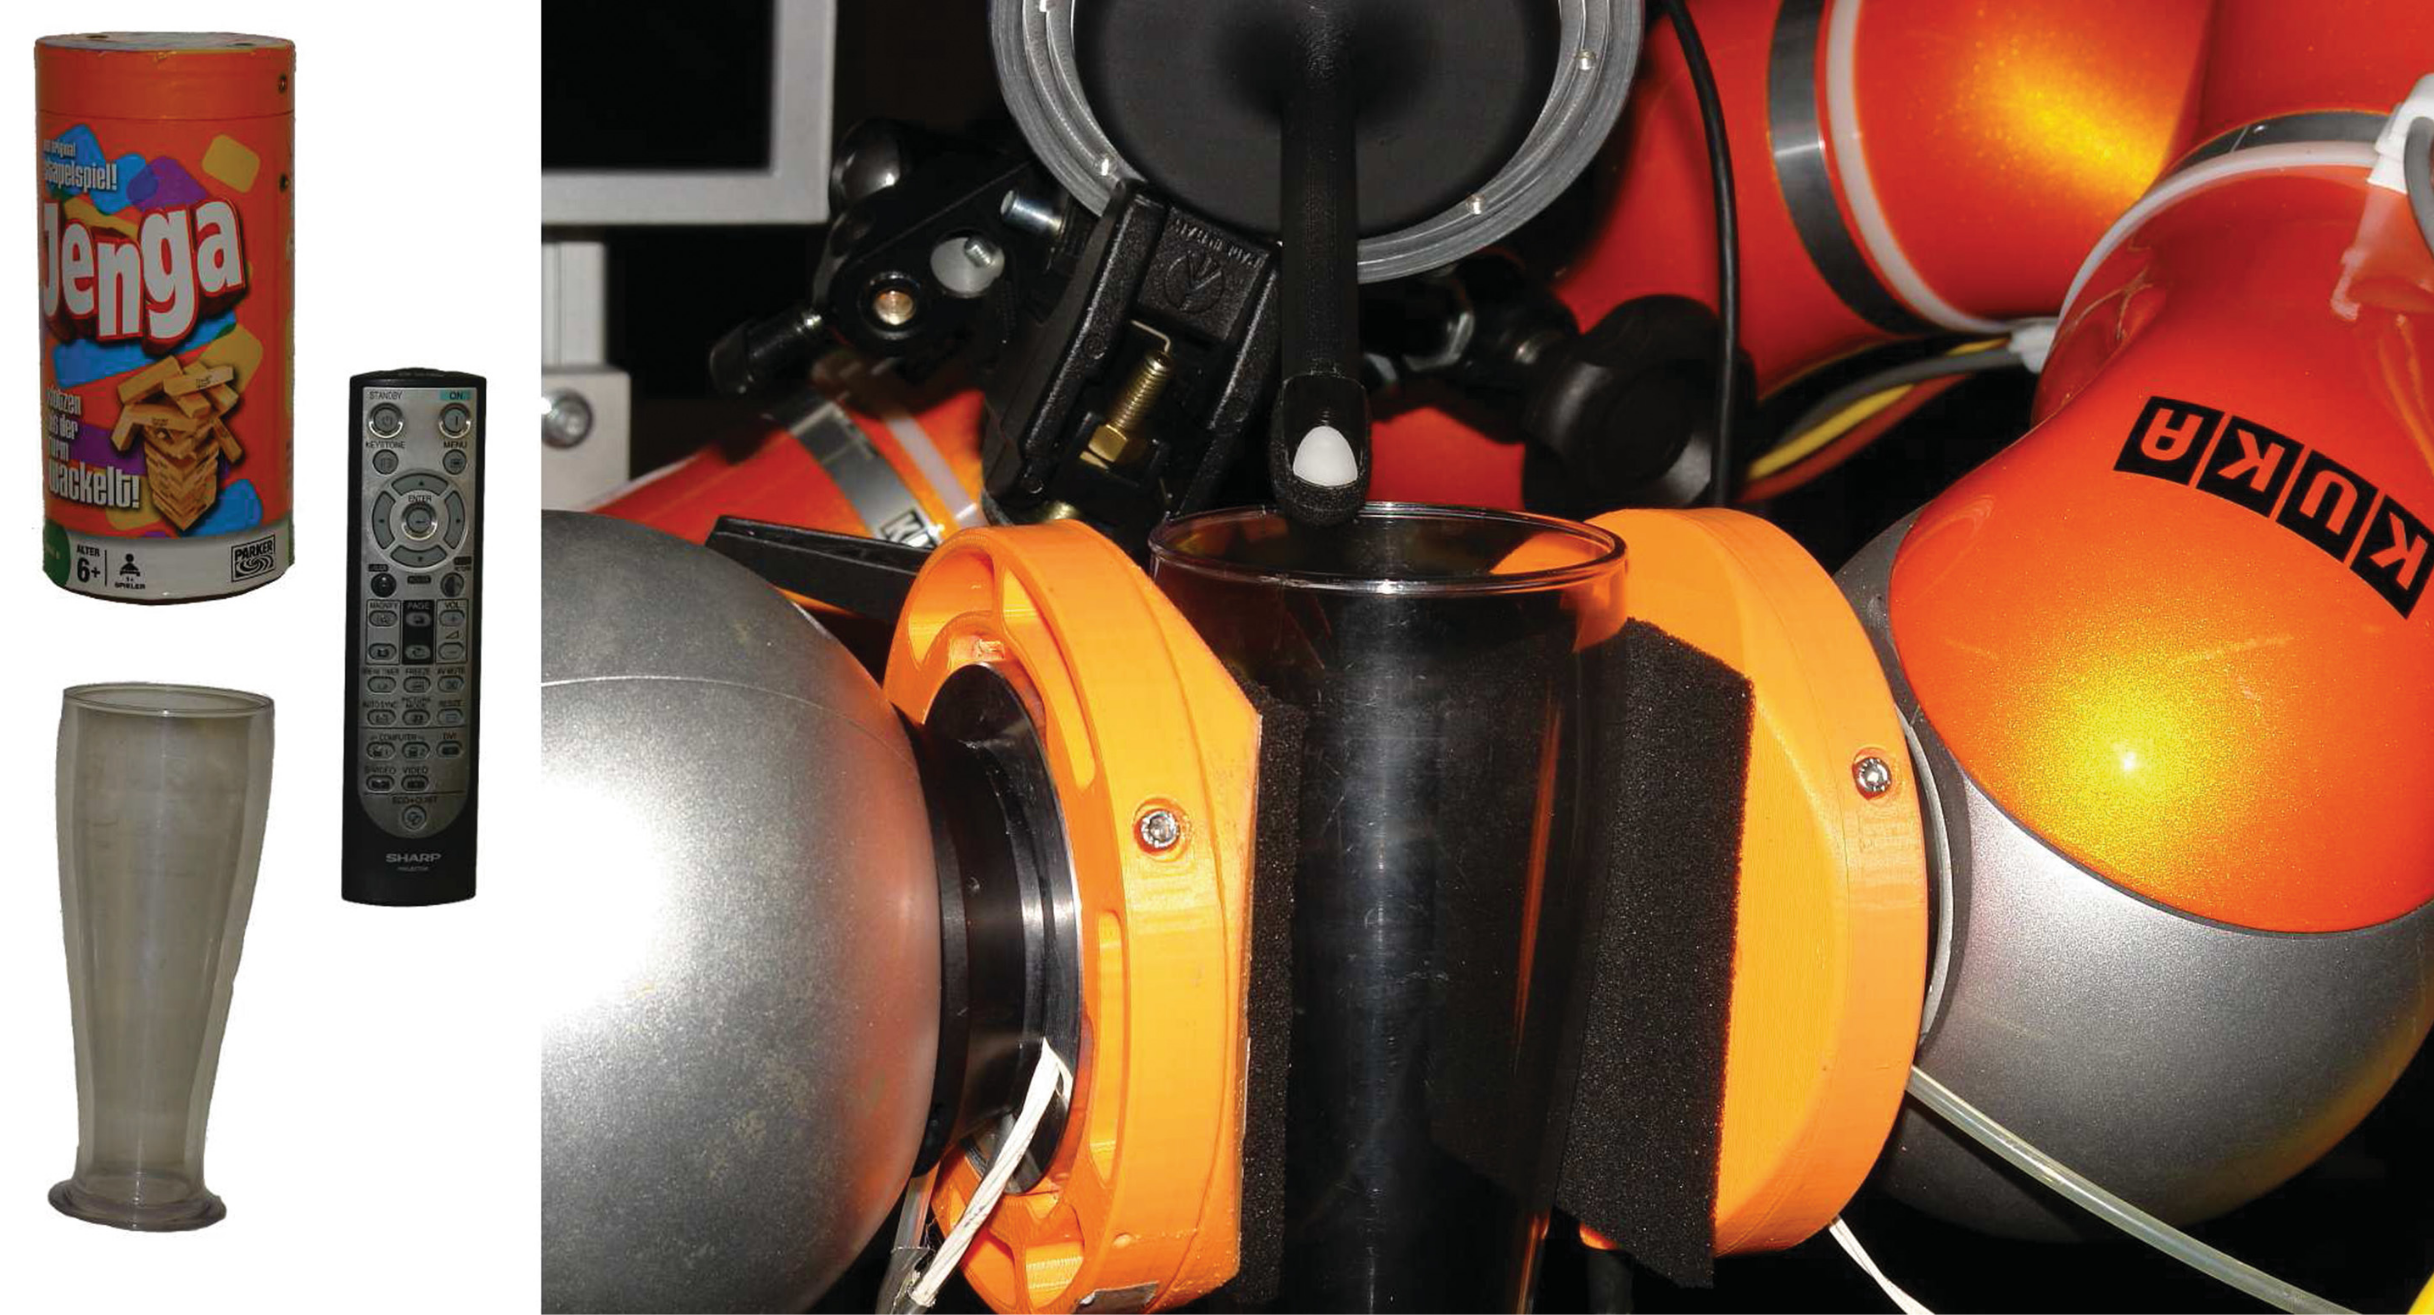
\includegraphics[width=\linewidth]{Figures/Tactile/meier2016.png}
    \caption{Objects and robotic setup of Meier \emph{et al.} approach \cite{Meier2016a}. Three different objects were used for training and evaluation: a can, a remote controller, and a glass. Two KUKA LWR robots with piezo-resistive sensor arrays are used to hold a glass. Figure extracted from \cite{Meier2016a}.}
    \label{fig:tactile:meier2016}
\end{figure}

In contrast, Cockbum \emph{et al.} \cite{Cockbum2017} proposed to use autoencoders to calculate the relevant characteristics for the task. Afterwards, a dictionary of basis features was built using a sparse encoding algorithm. Finally, the authors trained a \ac{SVM} in order to predict grasp stability using the dictionary. Similarly, Kwiatkowski \emph{et al.} \cite{Kwiatkowski2017} built a composite image by placing the readings of two matrix-like sensors side by side. Then, they used this tactile image as input for a \ac{CNN} along with the proprioceptive data from the robot. As a result, the proposed method calculated by itself the features needed for predicting grasp stability. Both of them used the same sensor (shown in Figure \ref{fig:tactile:kwiatkowski2017}): a custom-built array of $4\times 7$ tactels which rely on capacitive sensing to acquire static and dynamic variations in pressure over time.

\begin{figure}[!htb]
    \centering
    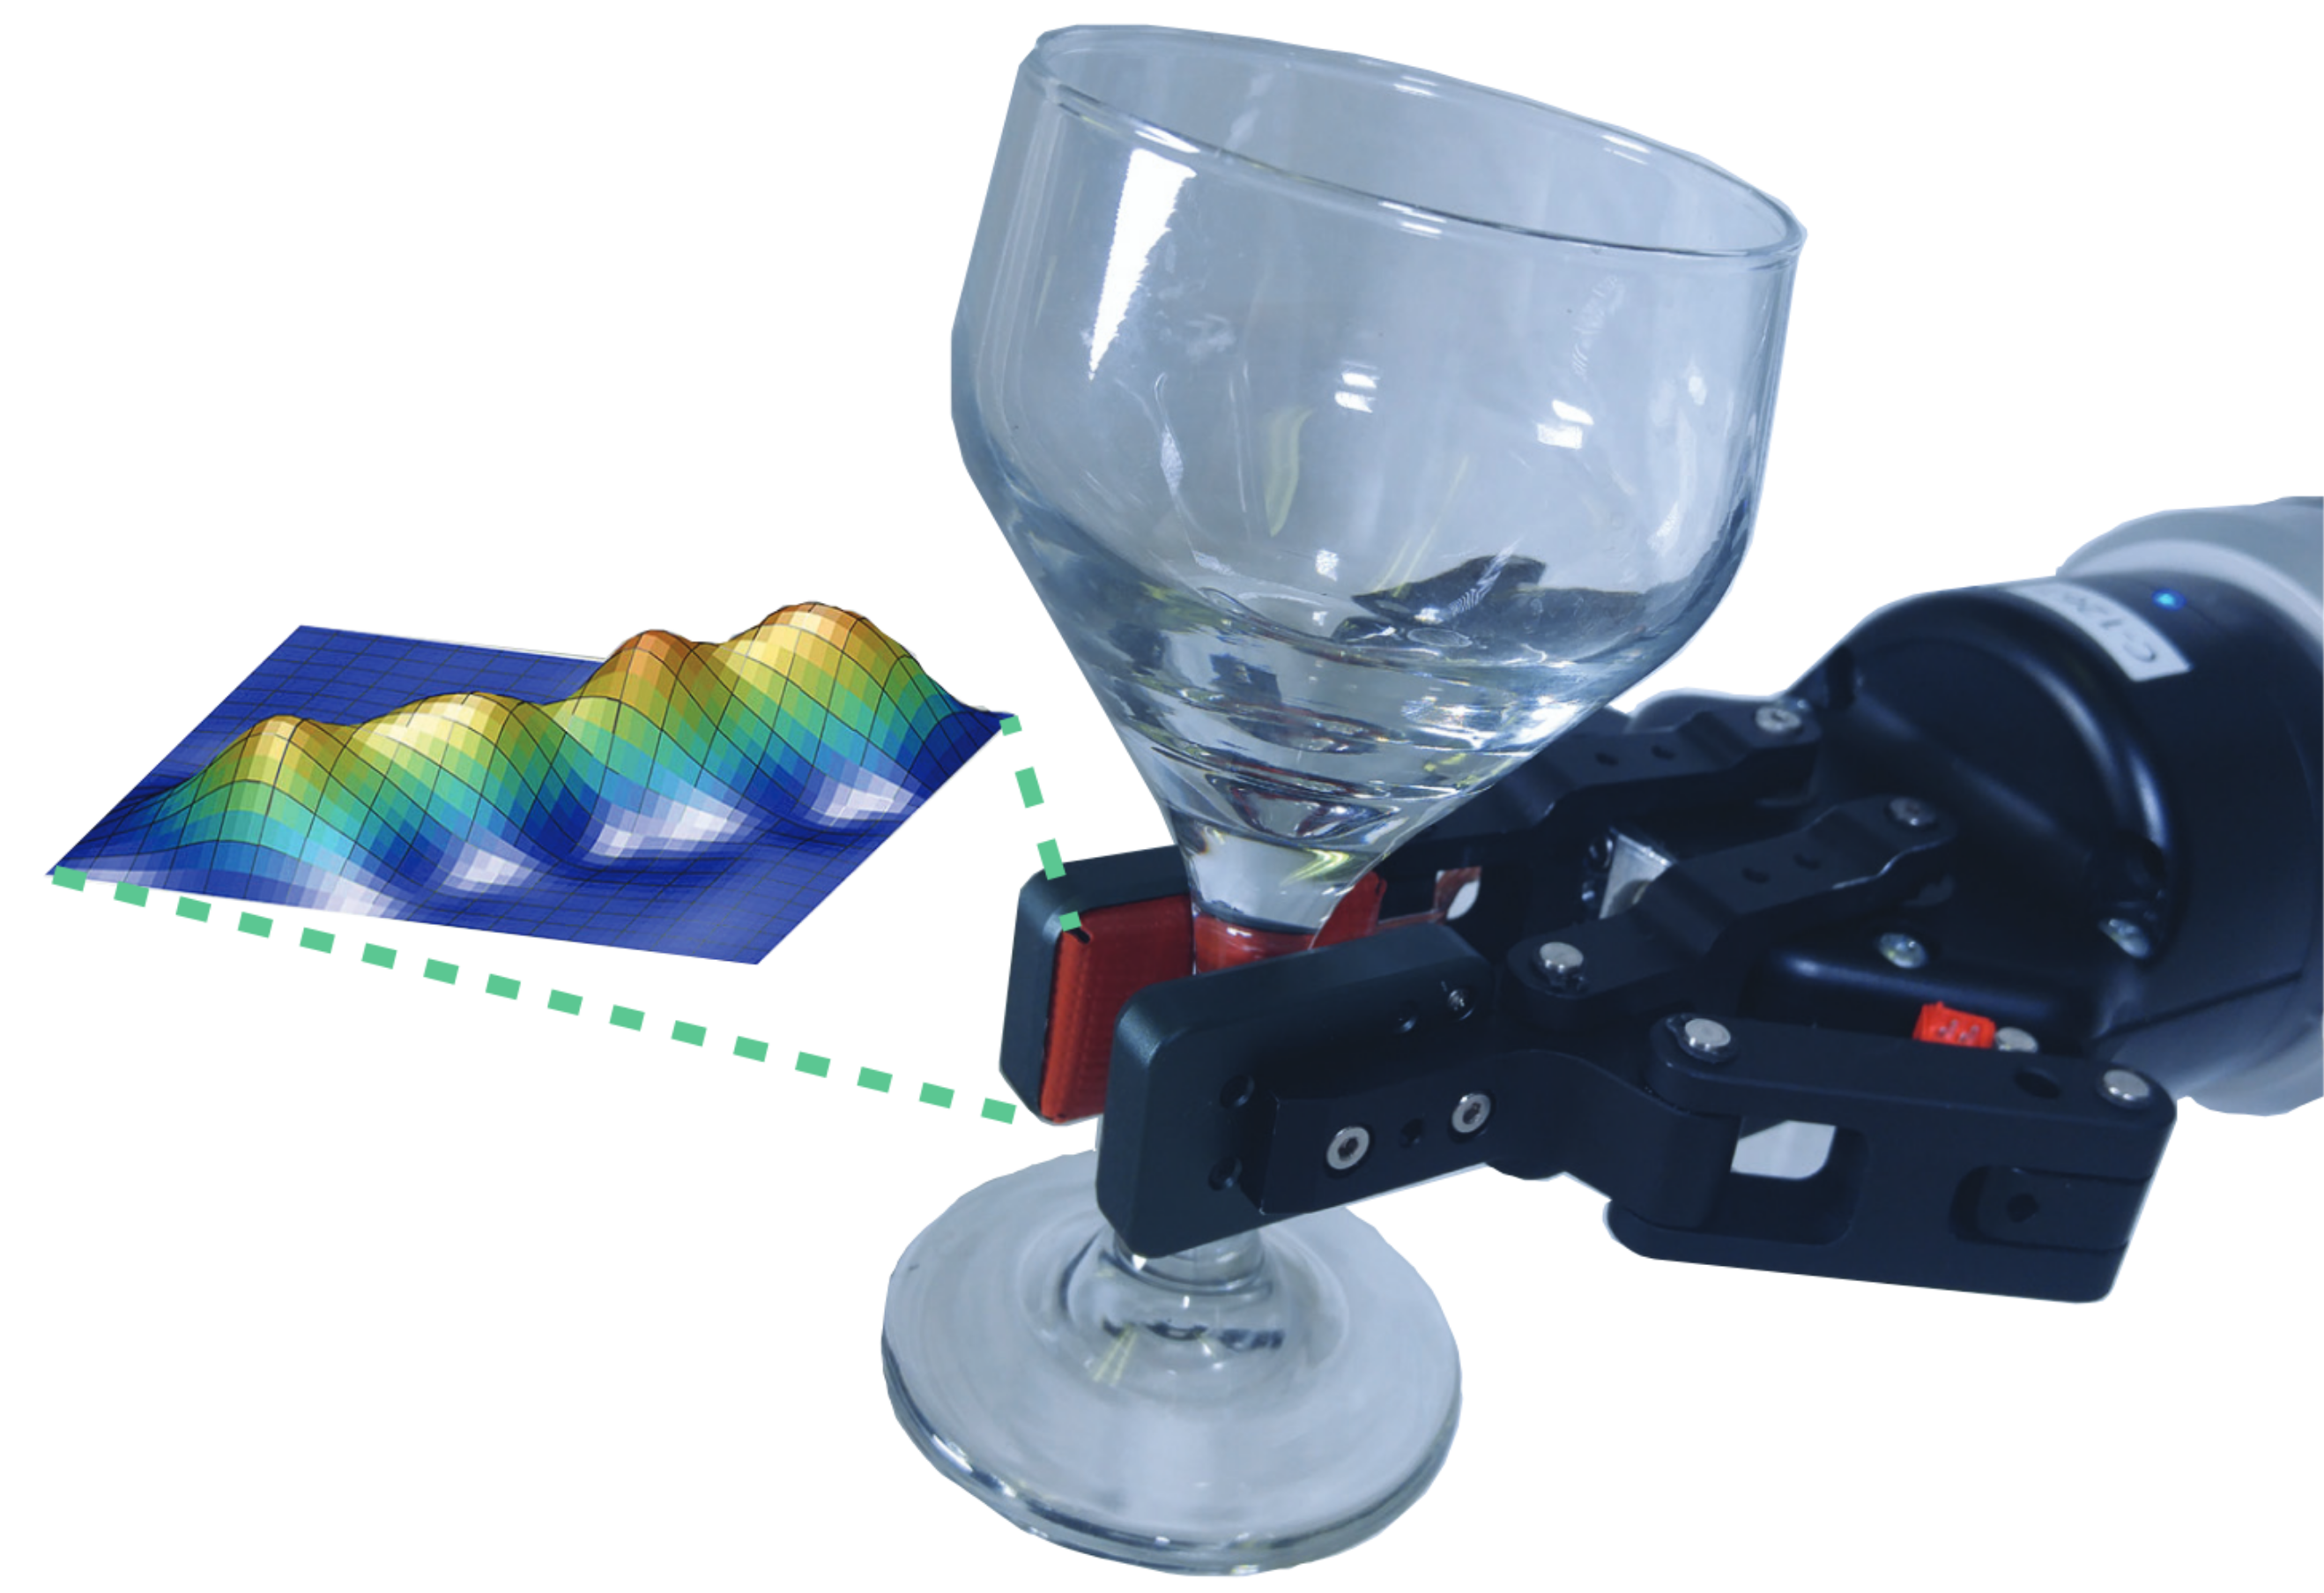
\includegraphics[width=0.8\linewidth]{Figures/Tactile/cockbum2017.png}
    \caption{Custom-built robotic gripper, used by Cockbum \emph{et al.}\cite{Cockbum2017} and Kwiatkowski \emph{et al.}\cite{Kwiatkowski2017}, with tactile sensors grasping a glass and the corresponding pressure image generated by one of them. Figure extracted from \cite{Kwiatkowski2017}.}
    \label{fig:tactile:kwiatkowski2017}
\end{figure}

There is an obvious trend in the field that suggests the interpretation of tactile sensors as images in order to exploit the potential of \ac{CNN} as spatial feature learners. In certain cases, even vision-based sensors are used for this purpose. Calandra \emph{et al.} \cite{Calandra2017} used a tactile sensor that contained an internal camera which recorded the deformation of the gel inside the sensor due to its contact with a surface. Some examples of tactile images collected by this sensor, namely GelSight, are shown in Figure \ref{fig:tactile:calandra2017}. The recorded tactile images were utilized to train a \ac{CNN} in order to predict the grasp outcome.

\begin{figure}[!htb]
    \centering
    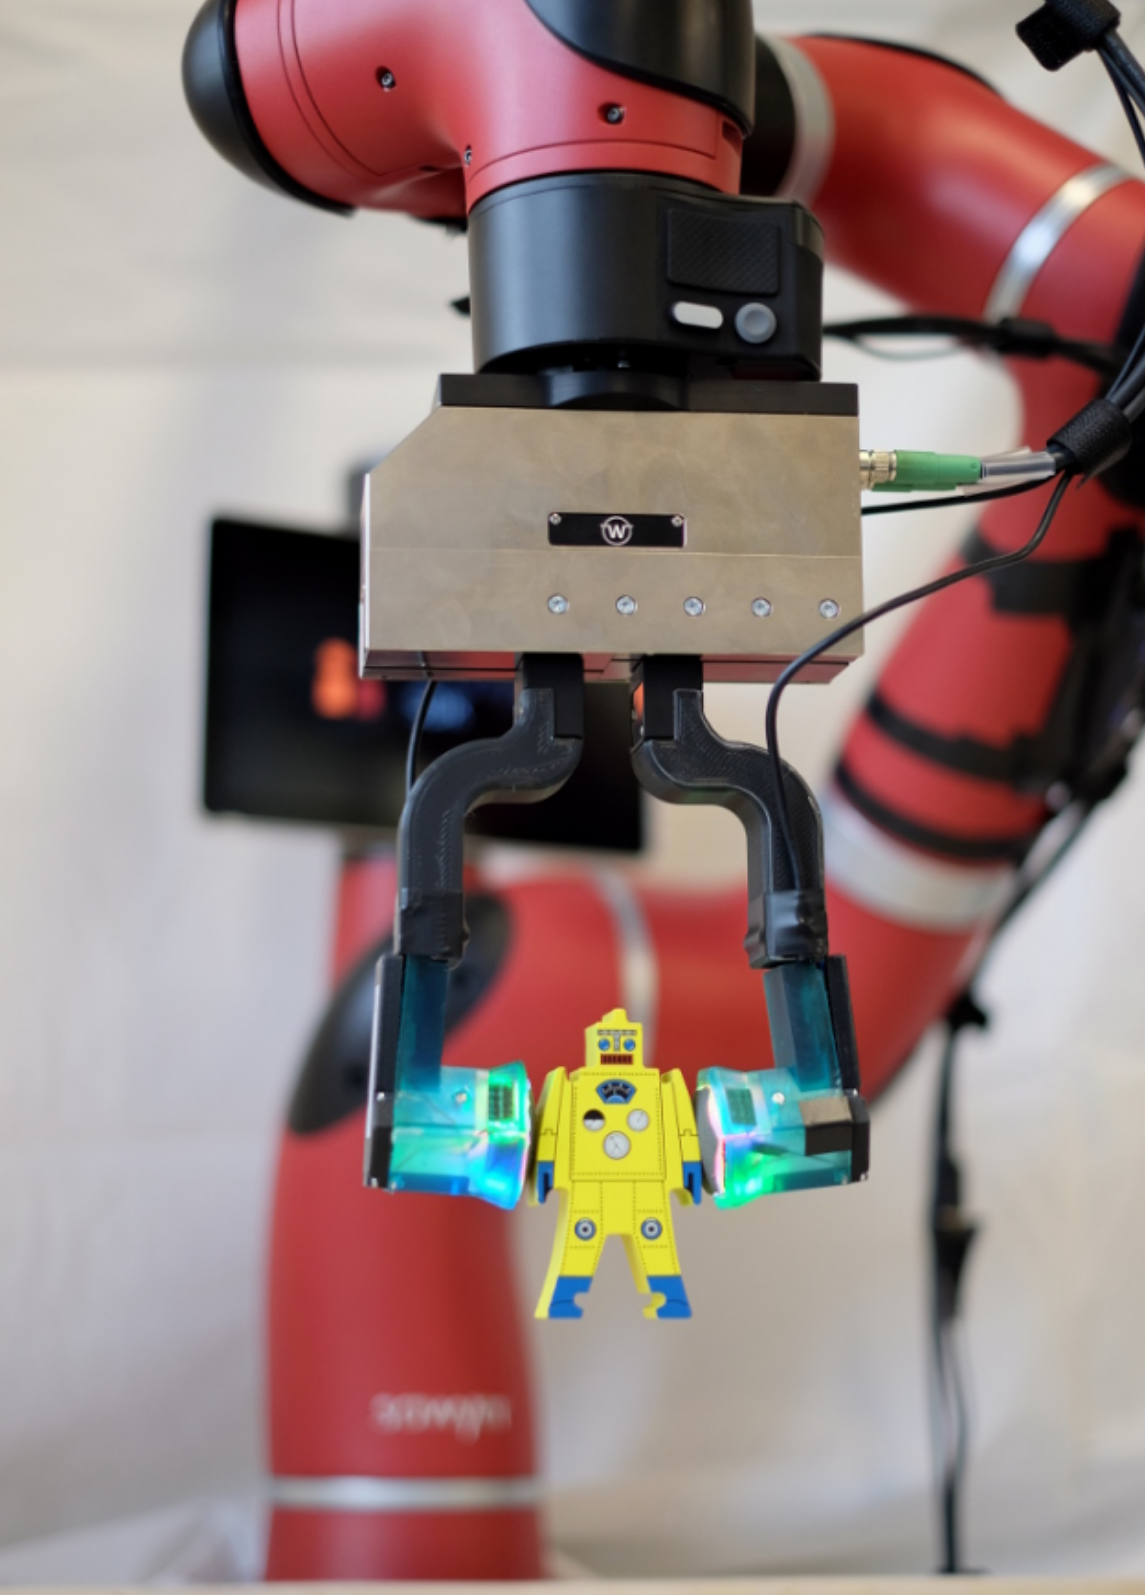
\includegraphics[width=0.21\linewidth]{Figures/Tactile/calandrarobot.png}
    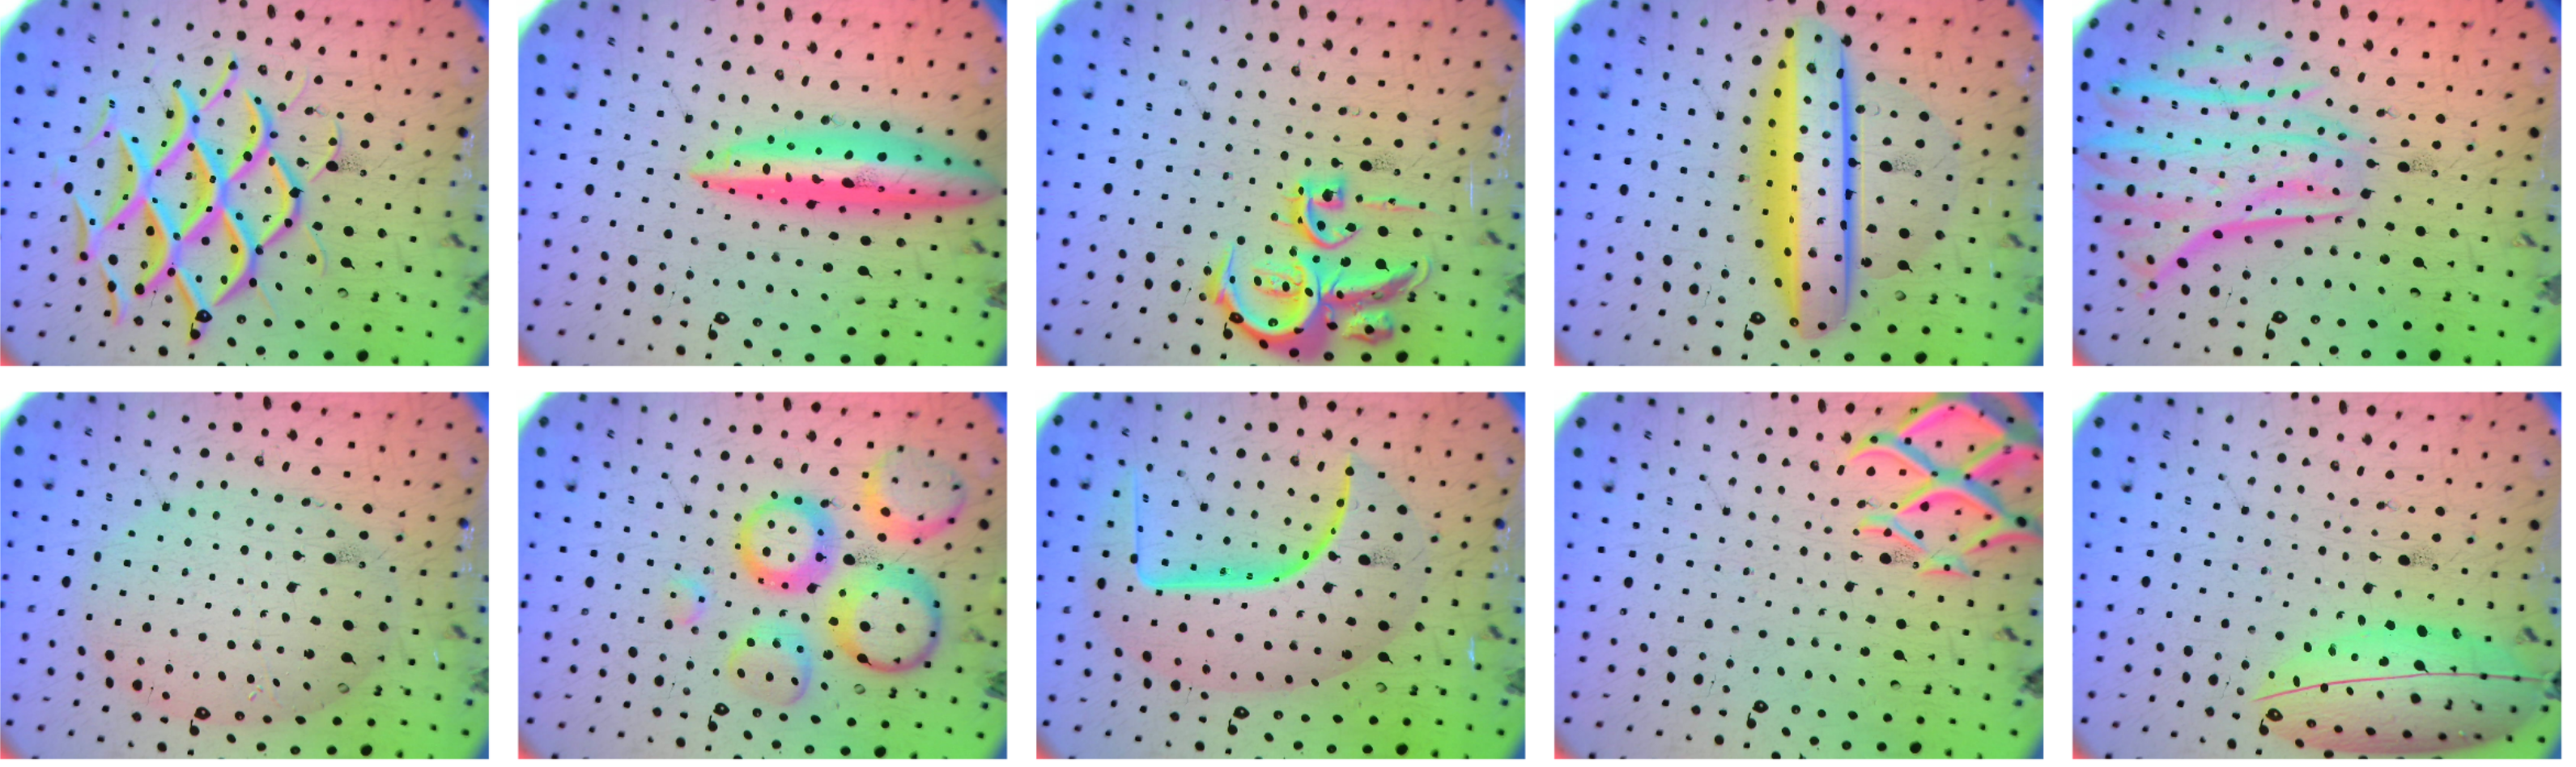
\includegraphics[width=0.78\linewidth, clip, trim=0 0 700 0]{Figures/Tactile/calandragelsight.png}
    \caption{Robotic gripper used by Calandra \emph{et al.}\cite{Calandra2017} and examples of raw tactile data capture by the custom-built GelSight camera embedded inside the tactile sensor. Figure extracted from \cite{Calandra2017}.}
    \label{fig:tactile:calandra2017}
\end{figure}

In some other cases, the tactile sensor is not naturally arranged in an array or it does not contain a camera. This is the case of the BioTacSP sensor \cite{Syntouch2018}. In this case, it is necessary to devise an arrangement and preprocess the tactile readings in order to generate a tactile image which can be fed to a \ac{CNN}. Zapata-Impata \emph{et al.} \cite{Zapata2018} studied how the readings from a non-matrix like sensor should be arranged in a matrix in order to train a \ac{CNN} for grasp stability prediction (see Figure \ref{fig:tactile:impata2018}). Although such approach showed promising results, the spatial distribution of the sensor was not accurately reflected because it reduced the \acs{3D} locations of the tactels into \acs{2D} coordinates of a tactile image.

\begin{figure}[!htb]
    \centering
    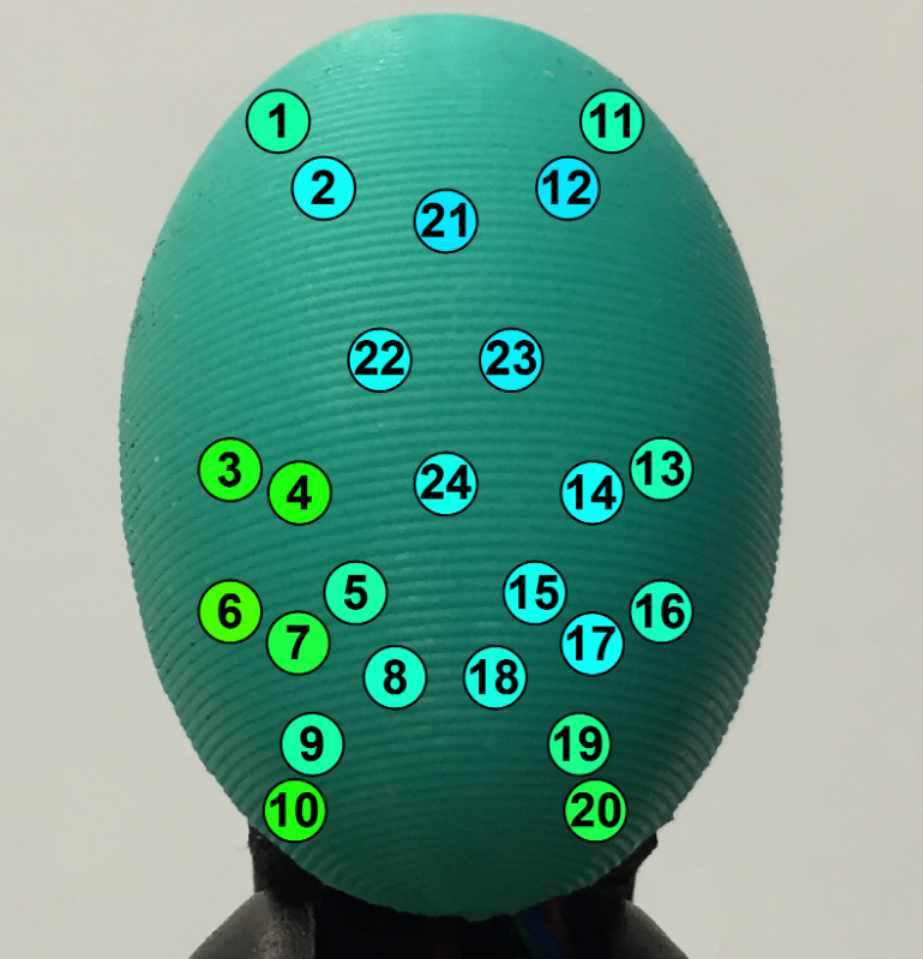
\includegraphics[width=0.3\linewidth]{Figures/Tactile/tactilebrayan1.png}
    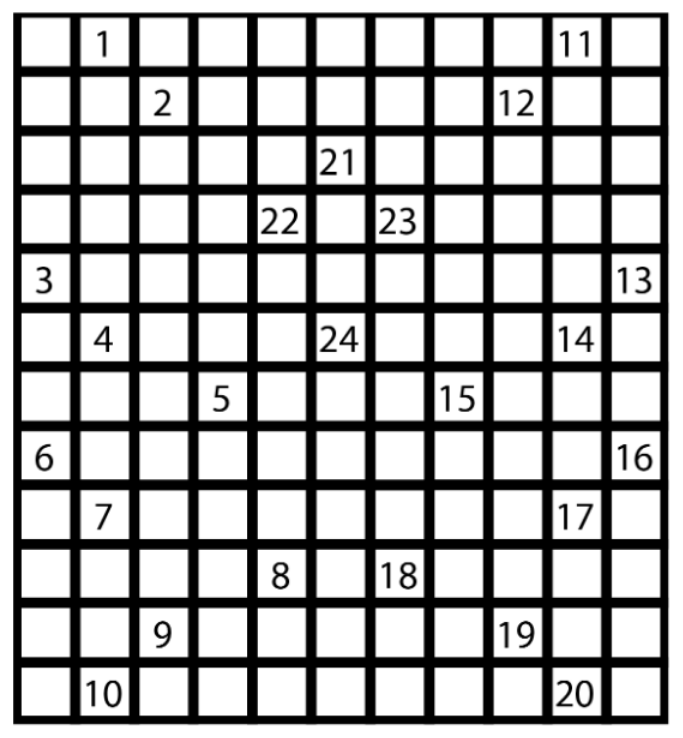
\includegraphics[width=0.3\linewidth]{Figures/Tactile/tactilebrayan2.png}
    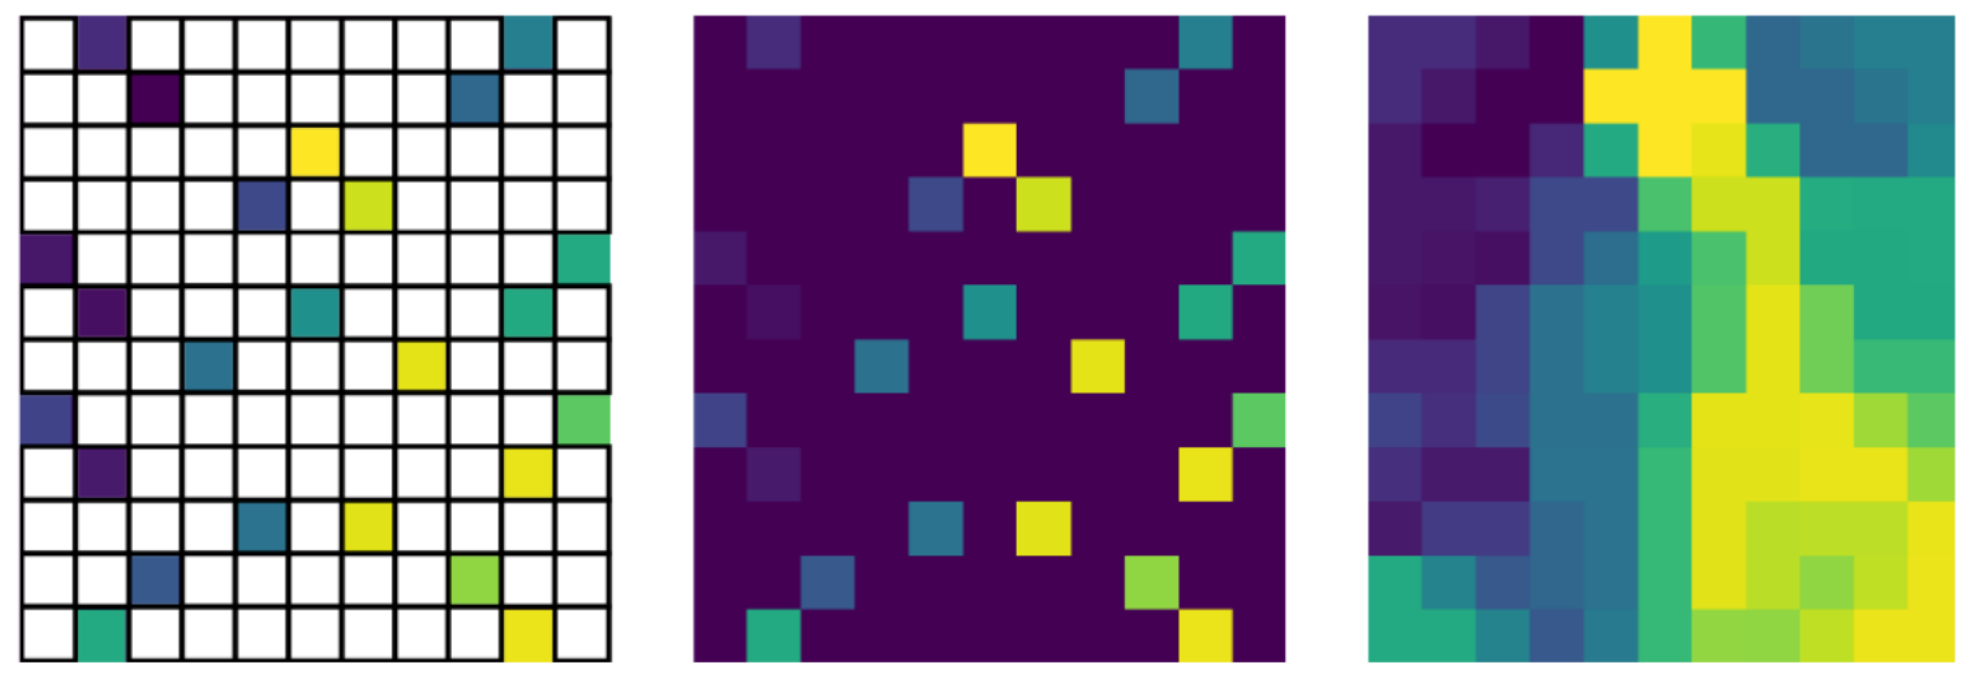
\includegraphics[width=0.7\linewidth]{Figures/Tactile/tactilebrayan3.png}
    \caption{BioTacSp sensor used by Zapata-Impata \emph{et al.} and the corresponding tactile images generated from the sensor readings using a custom arrangement. Figure extracted from \cite{Zapata2018}.}
    \label{fig:tactile:impata2018}
\end{figure}

Recently, a novel trend aims to combine \acp{CNN} with \acp{LSTM} for grasp stability prediction to make them able to process spatio-temporal information. The hypothesis states that, although static information can be successfully used to predict stability, more useful information to better discriminate between stable and unstable grasps can be learnt from temporal data, e.g., whether the object is moving at a dangerous speed. Li \emph{et al.} \cite{Li2018} learnt visual features from a camera-based tactile sensor, similar to the one used by Calandra \emph{et al.} \cite{Calandra2017}, and an external camera pointing towards the scene. These features were calculated using a pre-trained \ac{CNN}. Then, both cameras features were concatenated and passed as time sequences to an \ac{LSTM}, which was in charge of predicting slippage. Similarly, Zhang \emph{et al.} \cite{Zhang2018} used another camera-based tactile sensor for grasp stability detection but in this work the authors trained a \ac{ConvLSTM} and they only passed the sensor images to the network.

\subsection{Grasp Stability Datasets}

\subsection{Graph Neural Networks}
\label{cha:tactile:sec:relatedworks:subsec:gcns}

Lately, \acp{GNN} have emerged as a solid alternative to process irregular data which can be structured as graphs. Their original focus was tasks whose data can be expressed as graphs holding locality, stationarity, and composionality principles in general. In the literature, various works have successfully made use of this kind of architecture to deal with unstructured \acs{3D} representations mainly in classification tasks. Most of them  have proposed extensions to the well-known \ac{CNN} architecture to process graph-structured data. That generalization is not trivial since various problems must be addressed when applying convolution filters in domains in which there is no regular structure. In that regard, there are two dominant ways to convolve a graph signal with a learned filter: spatial or spectral.

Spectral methods are characterized by providing a spectral graph theoretical formulation of CNNs on graphs using Graph Signal Processing (GSP) theory \cite{Shuman2013}. The fundamentals of this kind of methods rely on decomposing the graph Laplacian to form a Fourier basis via an eigendecomposition of the graph matrix, i.e., a spectral decomposition. By doing that, a convolution in the graph domain can be expressed as a multiplication in the spectral one. This kind of methods usually faces three challenges: the design of compactly supported filters, the definition of parameter sharing schemes among different graphs, and the aggregation of multi-scale information. Arguably, the most common and limiting drawback is the first challenge: filters are not directly transferable to different graphs. Since filters are learned in the context of the spectrum of the graph Laplacian, a global graph structure must be assumed. In other words, only the signals on the vertices may change, the structure of the graph must remain the same.

Spatial methods constitute the straightforward generalization of convolutions to graph, just by sliding a filter on the vertices as a traditional CNN does with any other structured data representation. Despite its simplicity, the direct application of the definition of a convolution to graphs poses two difficulties: the definition of neighborhoods, and the ordering of the nodes to form receptive fields. Because of that, one common problem of spatial methods is the difficulty to generate a weight sharing schema across graph locations due to the fact that local neighborhoods can be completely different, i.e., the number of nodes adjacent to another one varies and there is no well-defined ordering for them.

Here we briefly review the most relevant \acp{GNN} that have been successfully applied to similar problems to the one at hand.

The pioneer spectral formulation of a CNN to operate over irregular domains modeled as graphs was introduced by Bruna et al. \cite{Bruna2013}. In that work, they exploited the global structure of the graph with the spectrum of its graph-Laplacian to extend the convolution operator. This method was applied to hand-written digit classification using the \ac{MNIST} dataset.

Defferrard \emph{et al.} \cite{Defferrard2016} proposed strictly localized filters, which are provable to be localized in a ball of a certain radius, i.e., hops from a specific vertex. That enhancement has some other collateral effects such as improved computational complexity for the filters (linear w.r.t. the support’s size and the number of edges). They also introduced an efficient  pooling strategy based on a rearrangement of the vertices as a binary tree. Their approach, namely \emph{Chebyshev Spectral Graph Convolutional Operator} or just \emph{ChebConv}, was successfully applied and performed similarly to classical \acp{CNN} in digits classification problems such as \acs{MNIST}.

Kipf and Welling \cite{Kipf2016} introduced a set of simplifications to Bruna's \cite{Bruna2013} and Defferrard's \cite{Defferrard2016} formulations to improve performance and scalability in large-scale networks. They proved the efficacy of their work on transductive node classification on very large scale networks for various problems such as semi-supervised document classification in citation networks (citeSeer, Cora and PubMed datasets) and semi-supervised entity classification in a knowledge graph (\acs{NELL} dataset). As its main feature, their \emph{GCNConv} operator takes advantage of fast localized first-order features to achieve linear scaling in the number of graph edges.

Simonovsky and Komodakis \cite{Simonovsky2017}, inspired by the idea from Jia \emph{et al.} [3] about dynamic filter networks, took a similar approach for solving the weight sharing problem suffered by spatial methods. They introduced \acp{ECC} in which filter weights are conditioned on edge features and generated by a generator network. That generator, usually implemented as a \ac{MLP}, outputs specific weights for each edge in the neighborhood. That method was successfully tested on point cloud classification problems (Sydney urban objects and ModelNet), a standard graph classification benchmarks, and also on \acs{MNIST}.

Velickovic \emph{et al.} \cite{Velickovic2017} introduced a \emph{Graph Attention} operator, namely \emph{GATConv}, that leverages masked self-attentional layers to compute the hidden representations of each node in the graph, by attending over its neighbors, following a self-attention strategy. This approach addressed many of the key challenges of spectral-based methods and achieved or surpassed state of the art methods in the aforementioned citation network datasets as well as protein interaction ones.

Fey \emph{et al.} \cite{Fey2018} proposed the \emph{Spline-based Convolutional Operator}, a continuous and spatial kernel that leverages B-spline bases's properties to efficiently filter graph data of arbitrary dimensionality. They prove this method to be successful in digit image graph classification problems using \acs{MNIST} and graph node classification using the Cora dataset.

Following this success in those similar domains, we intend to use a \acs{GNN} to process tactile sensor readings and predict grasp stability. By doing so, we expect that such architecture is able to better capture the spatial locality and relationships of the tactile sensor readings expressed as graphs instead of other non-spatial (\acs{1D} arrays) or discrete (images) representations.

\section{TactileGCN}
\label{cha:tactile:sec:tactilegcn}

In this section, we describe our full approach for predicting grasp stability using tactile sensors. The whole pipeline comprises three main components:

\begin{enumerate}
    \item A robotic setup which consists of a Shadow hand and BioTac Sp sensors, all operated by \ac{ROS}.
    \item A tactile graph generator which takes the sensor readings and generates a proper graph representation for the network.
    \item A \ac{GNN} architecture to process such graphs and predict graph stability.
\end{enumerate}

\subsection{Robotic Set Up}
\label{cha:tactile:sec:tactilegcn:subsec:rpobotic-set-up}

In this work, we use the BioTac SP tactile sensors developed by Syntouch \cite{Syntouch2018}. The sensor provides three different sensory modalities: force, pressure, and temperature. In more detail, this biomimetic sensor counts with $24$ electrodes, also named taxels, integrated in just a single phalanx. These electrodes record signals from four emitters in the internal core of the sensor and, therefore, they measure the impedance in the fluid located between the internal core and the external elastic skin of the sensor. The fluid is displaced when the sensor makes contact with a surface, affecting that impedance read by the electrodes. Thus, the sensor can approximate how much pressure is being experienced at each electrode. In addition, the sensor features a hydro-acoustic pressure sensor in order to estimate a general pressure value and it also counts with a thermistor, which is used to detect vibrations and heat flows. The sensor is presented in Figure \ref{fig:biotac-sensor}.

\begin{figure}[!htb]
	\centering
	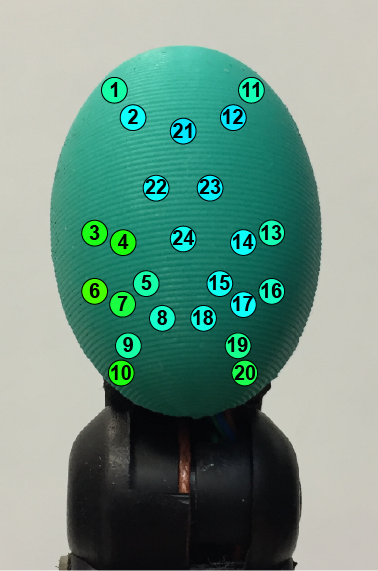
\includegraphics[width = 0.26\textwidth, clip = true, trim = 0 75 0 20]{Figures/Tactile/biotac-sensor.png}
	\caption{BioTac SP tactile sensor with its 24 electrodes approximated position.}
	\label{fig:biotac-sensor}
\end{figure}

For our work, we use a setup of three BioTac SP sensors in the tip of the index, middle finger, and thumb of a Shadow Dexterous robotic hand developed by the Shadow Robot Company \cite{ShadowRobotCompany2018}. The Shadow hand is an anthropomorphic hand with five fingers and $20$ \ac{DoF} in total. Those features allow the robot to reach a wide range of configurations that are comparable to those of a human hand. Its integration with the BioTac SP sensors is seamless since the sensor readings can be directly obtained using the \ac{ROS} \cite{Quigley2009} framework, in which the Shadow hand works.

\subsection{Tactile Graphs}
\label{cha:tactile:sec:tactilegcn:subsec:tactile-graphs}

In order to feed our \acl{GNN}, we expressed the aforementioned sensor readings in a novel graph representation, namely tactile graphs. Such graphs are triplet $G = (N, E, Y)$ where $N$ is a set of $24$ nodes ${n_0, ..., n_{23}}$ (one for each electrode or taxel in the sensor), $E$ is a set of ordered pair of vertices called edges, and $Y$ is the label or class of the graph (in our case, stable or unstable).

Each node $n$ in the graph $G$ represents a taxel and as such, they are characterized by a \acs{3D} position $p_n = (x_n, y_n, z_n)$ and a feature vector $f_n = (f_{n_0}, ..., f_{n_F})$ of arbitrary length $F$.

Node positions $p_n$ are accurately mapped to the physical taxel $(X, Y, Z)$ coordinates within the sensor. Such positions are specified in Table \ref{table:taxel_coordinates}. Edges or connections are generated following two different approaches: manual or \ac{k-NN}. For the first approach, we manually specified undirected connections following proximity and symmetry criteria. For the second one, we generated directed edges towards each \acl{k-NN} for each node. Figure \ref{fig:graph_3d} shows a \acs{3D} graph representation of a tactile graph.

\begin{table}[!htb]
    \centering
    \caption{Actual position of the taxels inside the BioTac SP sensor expressed in Cartesian coordinates $(X,Y,Z)$ in inches.}
    \begin{tabular}{lccc}
        \hline
        \textbf{Taxel} & \textbf{X (inches)} & \textbf{Y (inches)} & \textbf{Z (inches)}       \\
        \hline
        1     & 0.386434851  & -0.108966104 & 0.156871012  \\
        2     & 0.318945051  & -0.205042252 & 0.120706090  \\
        3     & 0.087372680  & -0.128562247 & 0.281981384  \\
        4     & 0.083895199  & -0.235924865 & 0.201566857  \\
        5     & -0.018624877 & -0.300117050 & 0.094918748  \\
        6     & -0.091886816 & -0.120436080 & 0.284956139  \\
        7     & -0.136659500 & -0.237549685 & 0.187122746  \\
        8     & -0.223451775 & -0.270674659 & 0.071536904  \\
        9     & -0.320752549 & -0.199498368 & 0.127771244  \\
        10    & -0.396931929 & -0.100043884 & 0.151565706  \\
        11    & 0.386434851  & -0.108966104 & -0.156871012 \\
        12    & 0.318945051  & -0.205042252 & -0.120706090 \\
        13    & 0.087372680  & -0.128562247 & -0.281981384 \\
        14    & 0.083895199  & -0.235924865 & -0.201566857 \\
        15    & -0.018624877 & -0.300117050 & -0.094918748 \\
        16    & -0.091886816 & -0.120436080 & -0.284956139 \\
        17    & -0.136659500 & -0.237549685 & -0.187122746 \\
        18    & -0.223451775 & -0.270674659 & -0.071536904 \\
        19    & -0.320752549 & -0.199498368 & -0.127771244 \\
        20    & -0.396931929 & -0.100043884 & -0.151565706 \\
        21    & 0.258753050  & -0.252337663 & 0.000000000  \\
        22    & 0.170153841  & -0.274427927 & 0.072909607  \\
        23    & 0.170153841  & -0.274427927 & -0.072909607 \\
        24    & 0.075325086  & -0.298071391 & 0.000000000\\
        \hline
    \end{tabular}
    \label{table:taxel_coordinates}
\end{table}

\begin{figure}[!htb]
	\centering
    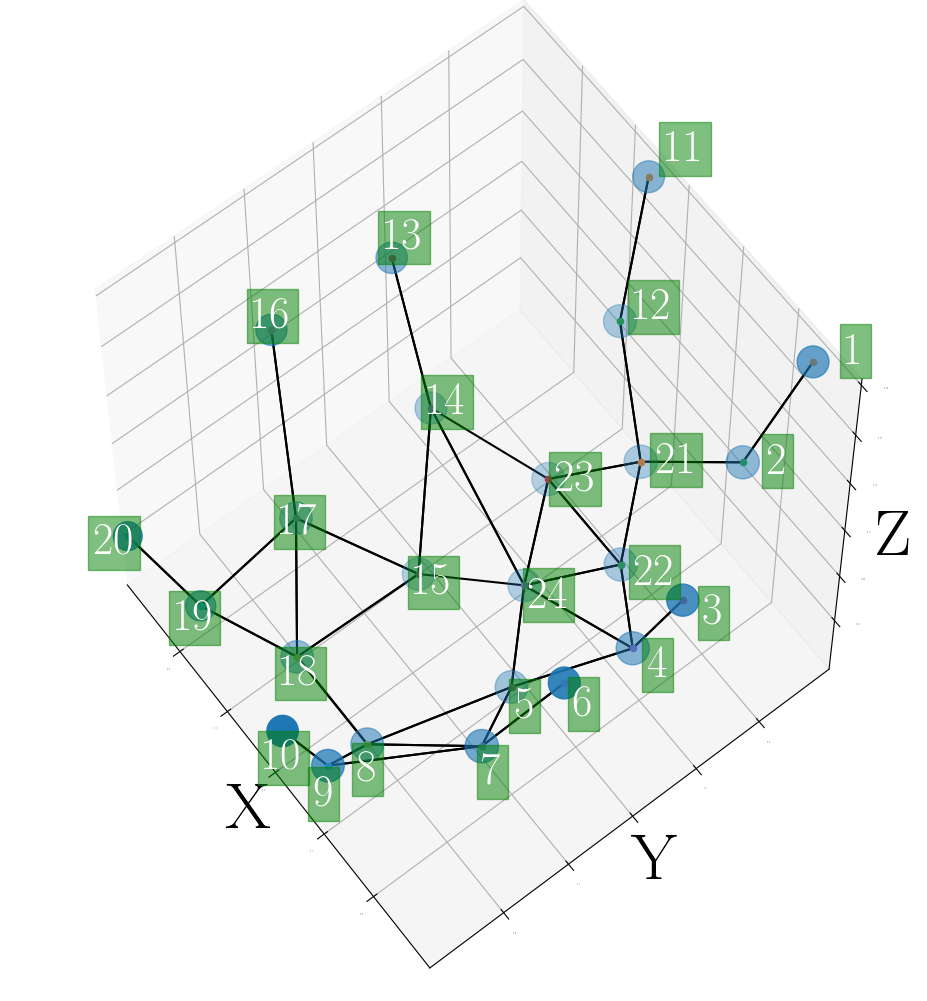
\includegraphics[width=0.8\linewidth]{Figures/Tactile/plot3d.png}
	\caption{3D visualization of the tactile graph layout using the accurate spatial arrangement from the actual BioTac SP sensor. Graph edges correspond to the manually defined connections.}
	\label{fig:graph_3d}
\end{figure}

Node features $f_n$ correspond to the taxel pressure readings. In the case of the most basic tactile graph, each node has three features, i.e., the pressure reading for each finger: index $f_{n_0}$, middle $f_{n_1}$, and thumb $f_{n_2}$. Figure \ref{fig:sample_graphs} shows visualizations of the three components of the feature vector for sample graphs generated with various values of $k=0$, $k=2$, $k=4$, $k=8$.

\begin{figure}[!htb]
    \centering
    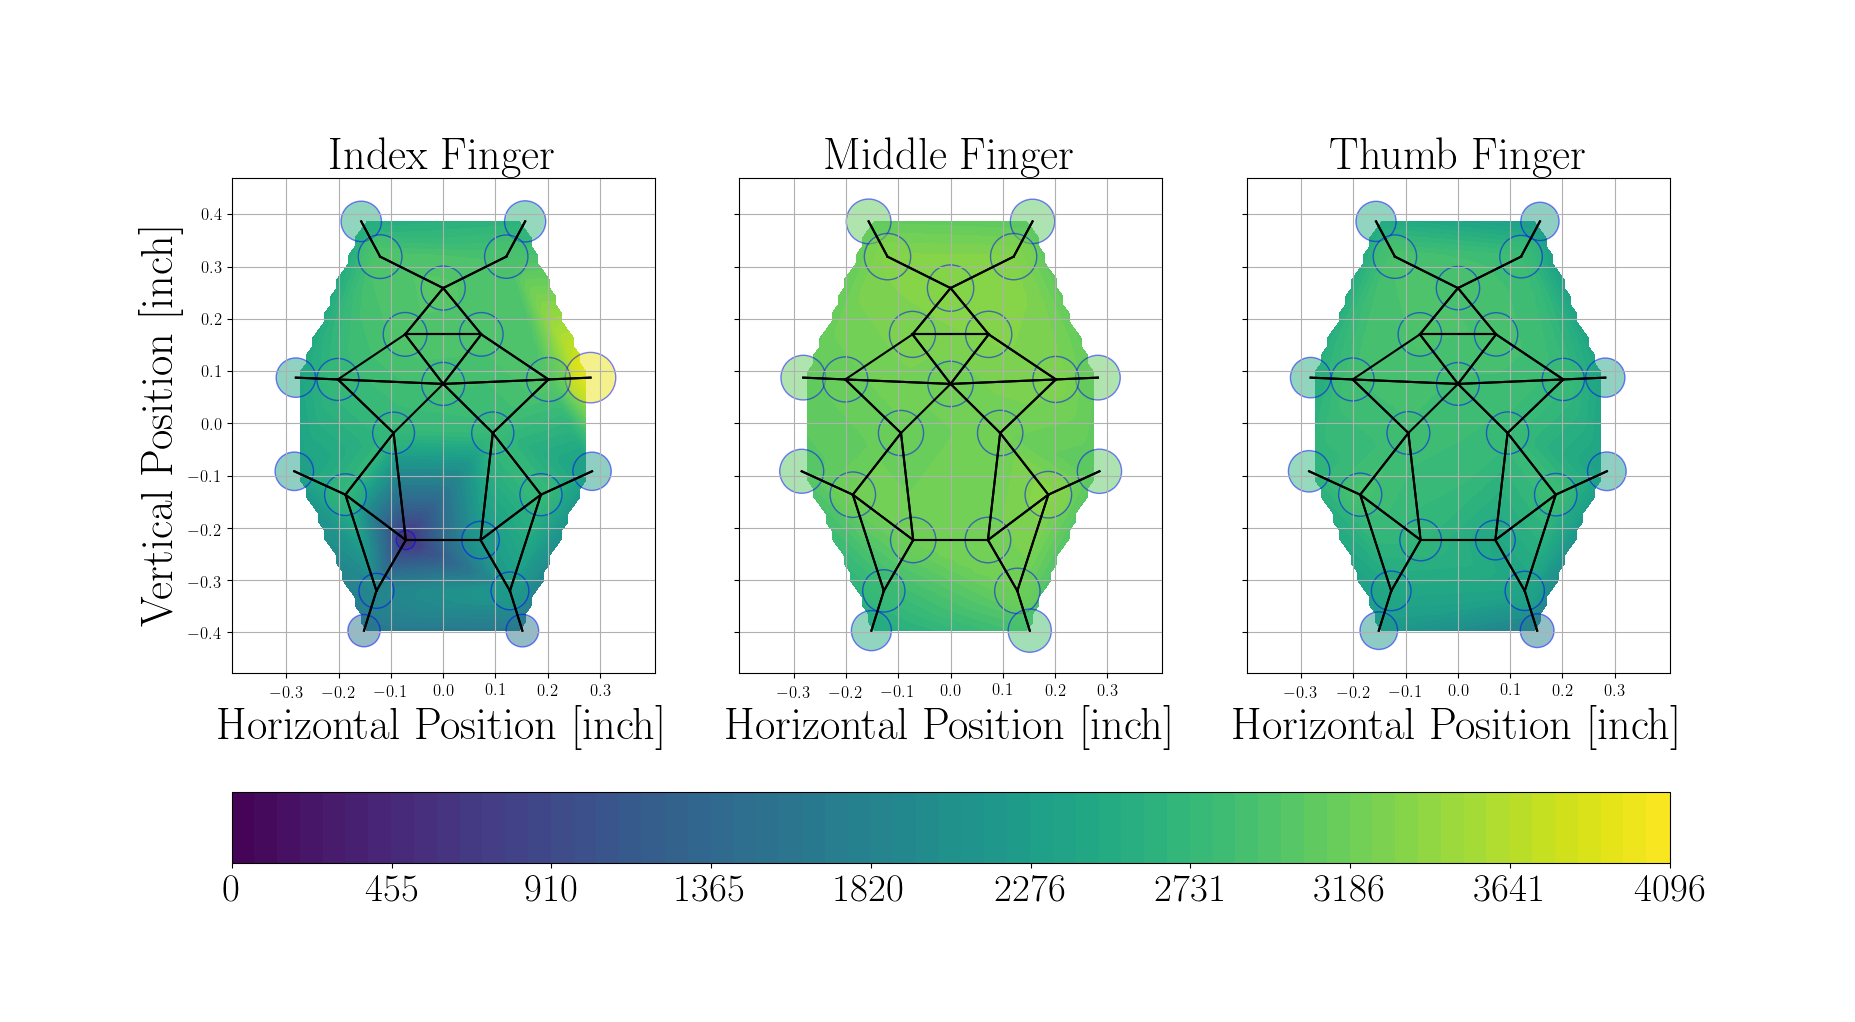
\includegraphics[width=\linewidth, clip, trim={90 170 80 50}]{Figures/Tactile/plot-k0.png}
    \bigskip
    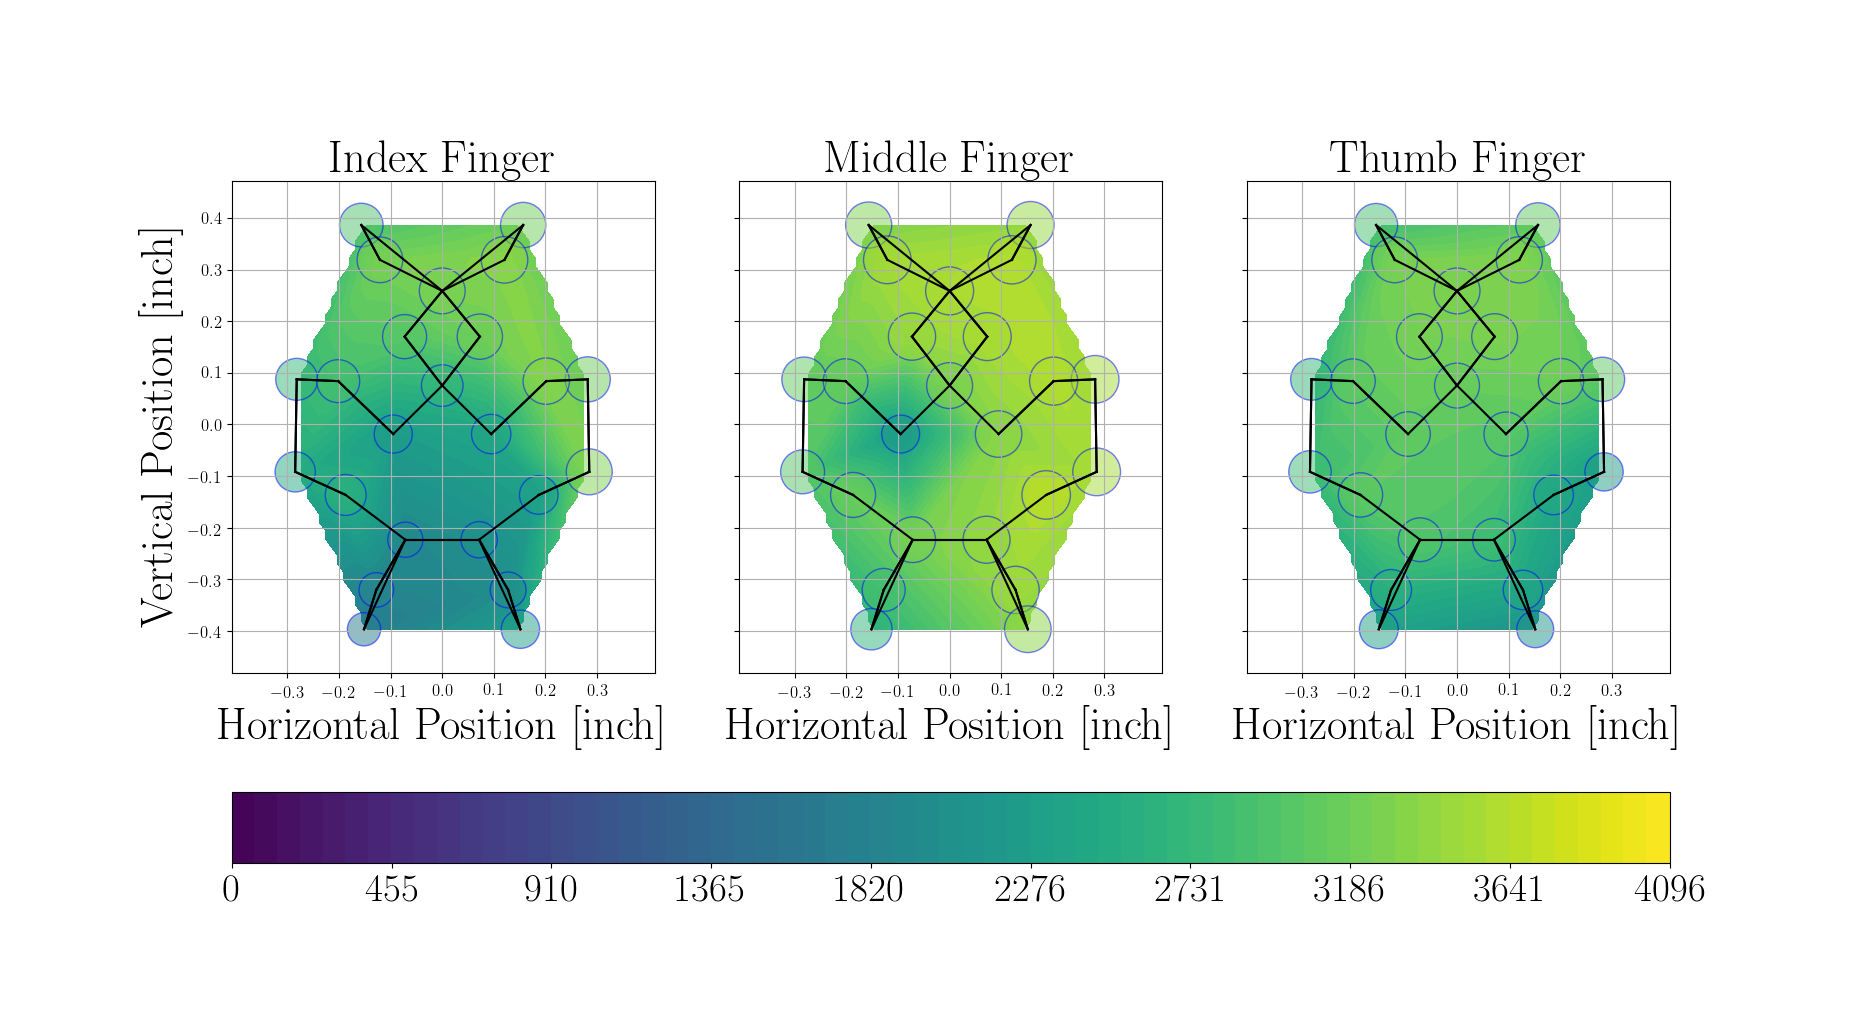
\includegraphics[width=\linewidth, clip, trim={90 190 80 50}]{Figures/Tactile/plot-k2.png}
    \bigskip
    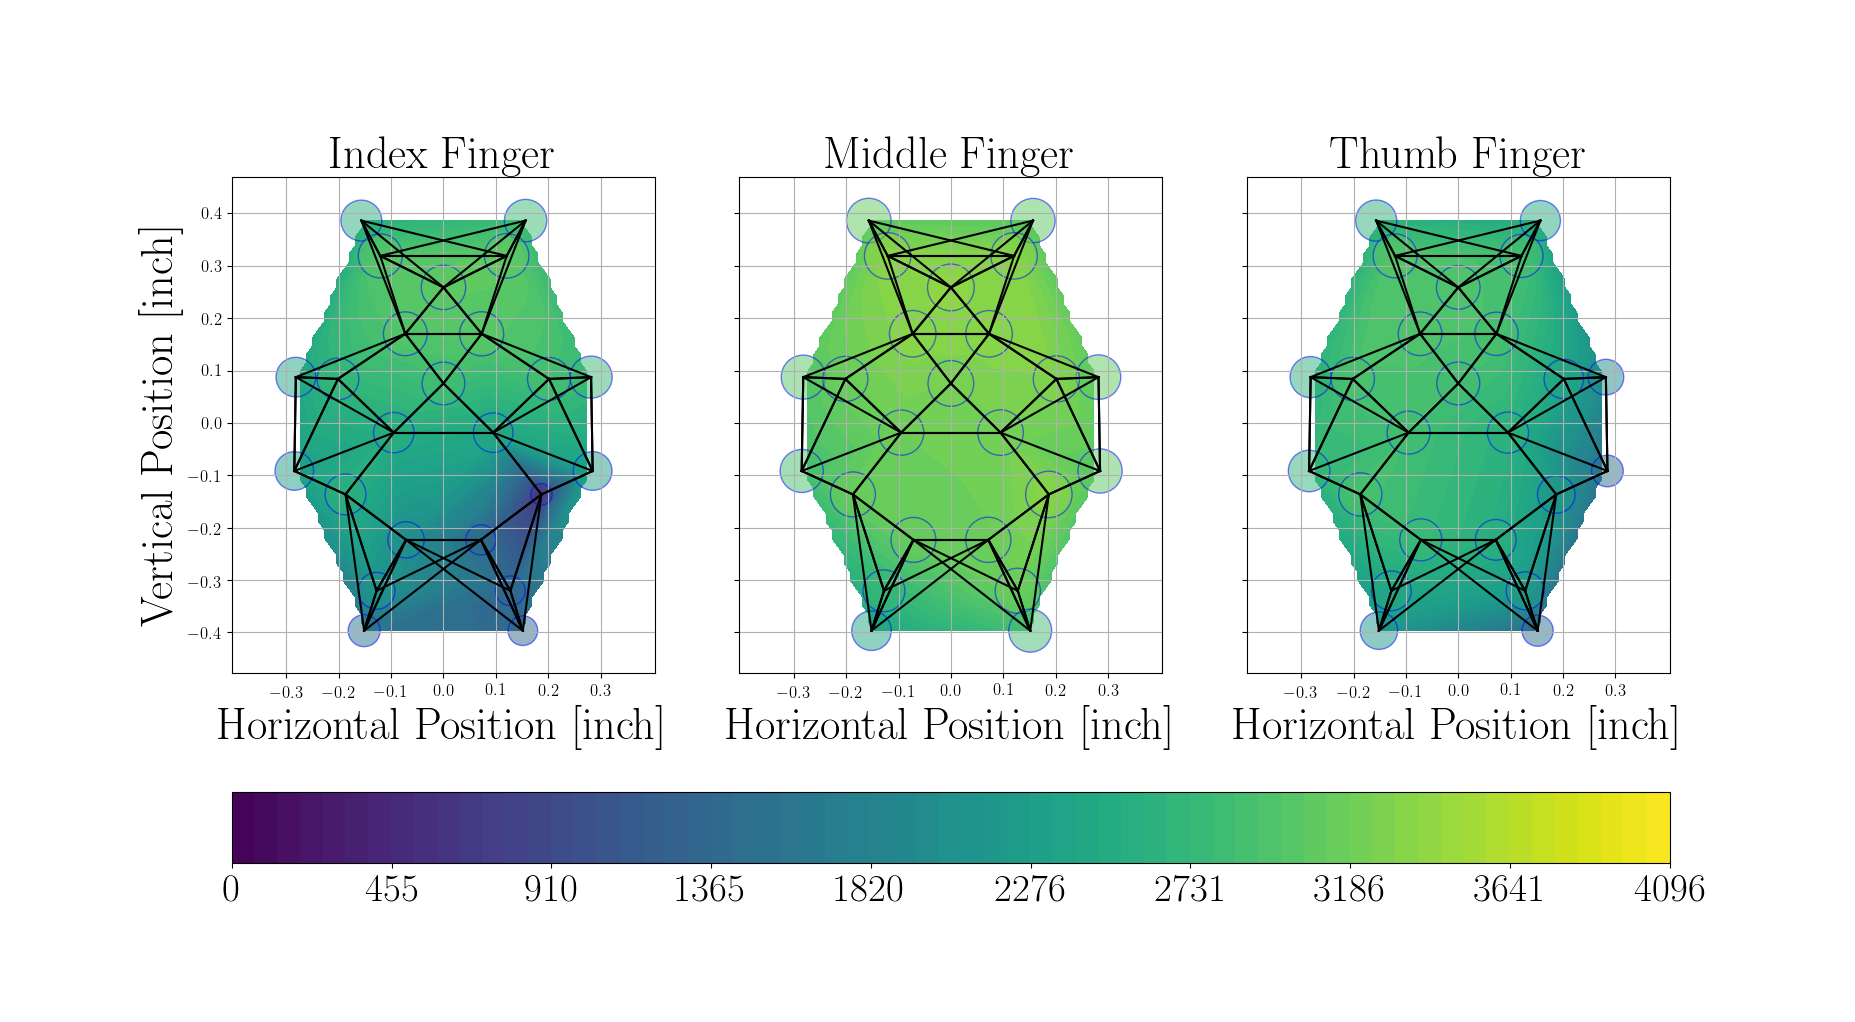
\includegraphics[width=\linewidth, clip, trim={90 190 80 50}]{Figures/Tactile/plot-k4.png}
    \bigskip
    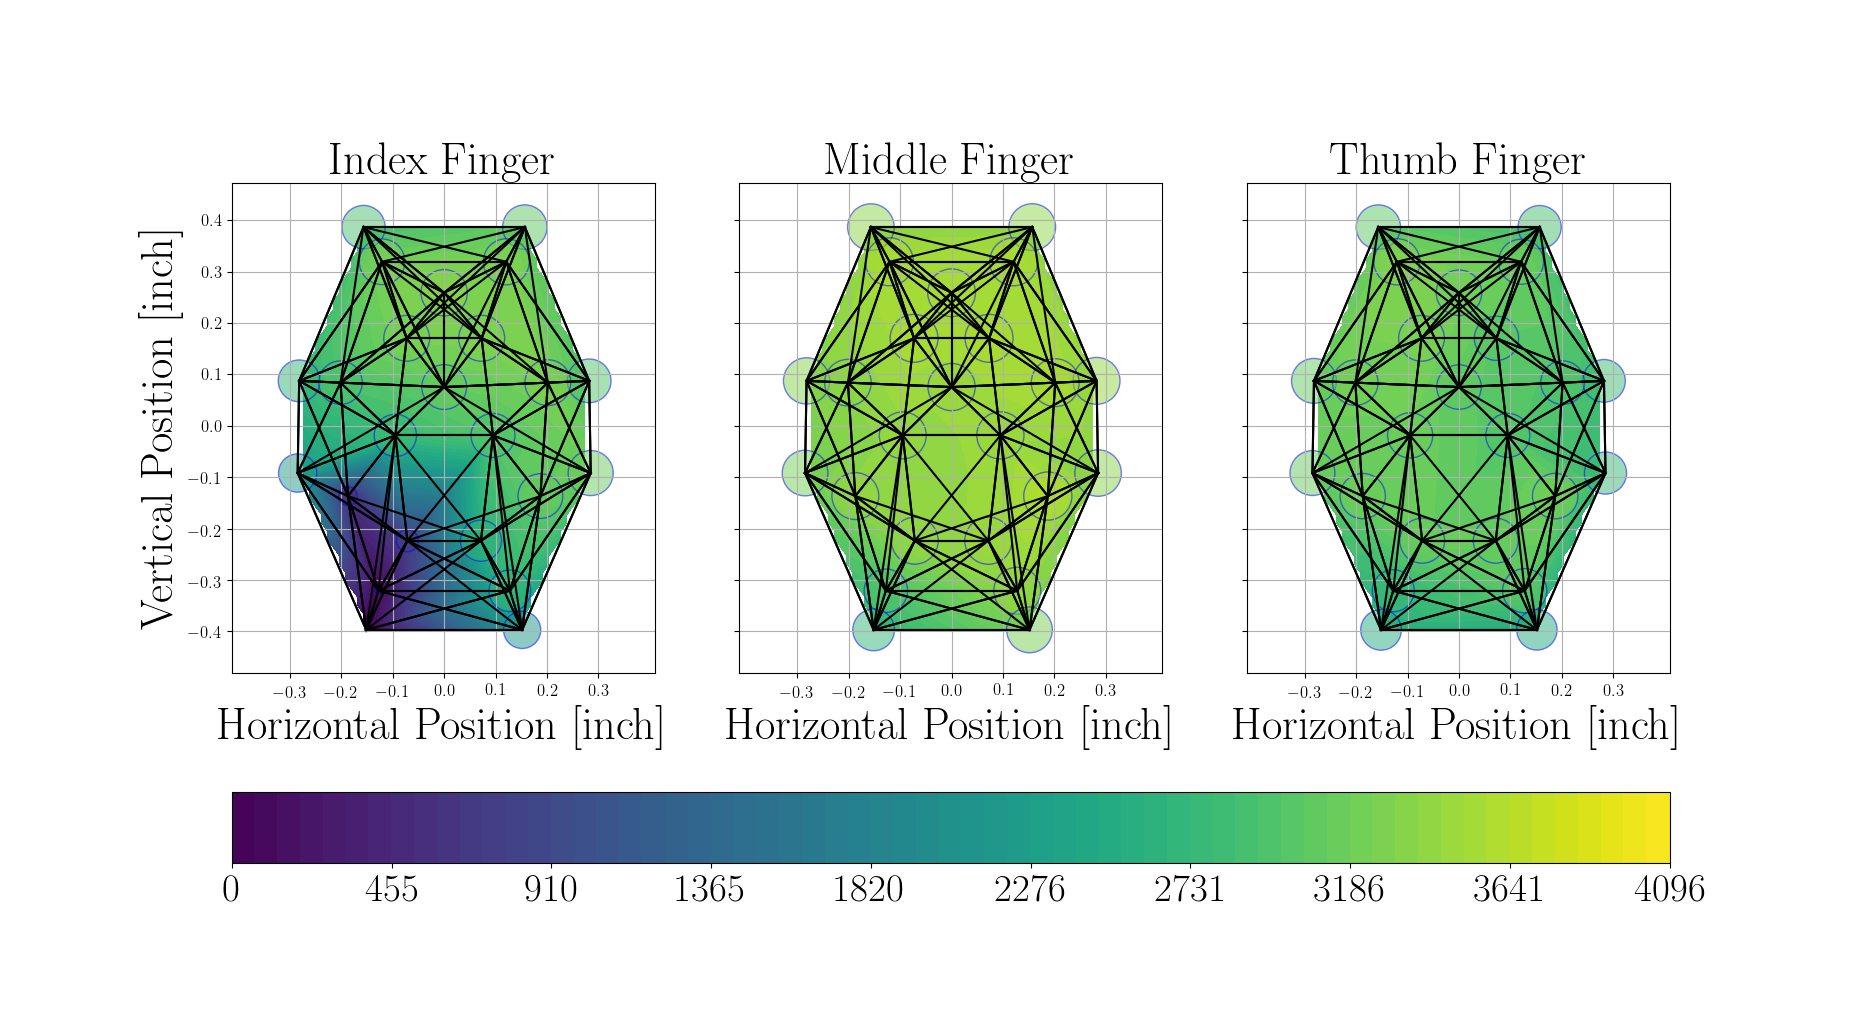
\includegraphics[width=\linewidth, clip, trim={90 10 80 50}]{Figures/Tactile/plot-k8.png}
	\caption{From top to bottom, undirected tactile graphs generated with various \ac{k-NN} configurations: $k=0$ (manually defined edges), $k=2$, $k=4$, and $k=8$. The three features (fingers) $f_{n_0}$, $f_{n_1}$, and $f_{n_2}$ are deocupled into three different plots and represented as contour plots in the XY plane. Nodes or taxels are shown as blue semi-transparent circles whose size depends on the pressure read on them. Undirected edges are represented by black lines. Features are color-coded in the range $[0, 4096]$.}
	\label{fig:sample_graphs}
\end{figure}

\subsection{\acl{GNN}}
\label{cha:tactile:sec:tactilegcn:subsec:gnn}

Our \acf{GNN} of choice is based on the \ac{GCN} model by Kipf and Welling \cite{Kipf2016}. Such model is arguably one of the most successful, yet simple, approaches to date to generalize a well-established model such as the \ac{CNN} to arbitrarily structured graphs \cite{Bronstein2017}\cite{Schlichtkrull2018}. Their proposal, which is somewhat similar to Defferard's \emph{et al.}, introduce a set of simplifications into a framework of spectral graph convolutions to make them train significantly faster and achieve state-of-the-art levels of accuracy across various classification tasks \cite{Defferrard2016}.

The goal of such models is to learn features on a graph $G = (N, E, Y)$ by taking as input a feature matrix $X$ ($N \times F$ with a feature vector $f_n$ for each node $n$) and a description of the graph structure in the shape of an adjacency matrix $A$ (computed from the set of edges $E$ in the graph). The output is another feature matrix $Z$ ($N \times F'$ with node-level feature vectors $f'_n$ with a predefined number of output features $F'$).

Each \ac{GCN} layer $H^(l)$ in a network with $L$ layers can be expressed as a non-linear function $H^{(l+1)} = f(H^{(l)}, A)$. The first layer takes the input feature matrix ($H^{(0)} = X$) and the final layer generates the output node-level feature matrix ($Z = H^{(L)}$). Each intermediate layer generates a node-level feature matrix $Z^{(l)}$ which is fed to the next layer. In the case of Kipf and Welling \cite{Kipf2016}, the graph-convolution layer $f(H^{(l), A)}$ is defined, in the most basic instantiation, as $\sigma(AH^{(l)}W^{(l)})$, where $\sigma$ is an activation function of choice and $W^{(l)}$ is the weight matrix for the $l$ layer.

This basic framework was heavily extended to overcome two limitations: (1) unless there are explicitly defined self-loops in the graph, the multiplication of $A$ only sums up the feature vectors of all the neighboring nodes but not the node itself, and (2) since $A$ is not normalized by default, the multiplication of $A$ has a huge impact on the scale of the feature vectors. Overcoming those two limitations is crucial to improve the model's convergence.

In order to fix those two limitations, they first enforced self-loops in the graph by adding the identity matrix to $A$ so the new adjacency matrix is $\hat{A} = A + I$. Secondly, they normalized that adjacency matrix in a row-like fashion by leveraging a symmetric normalization with the diagonal node degree matrix $\hat{D}$ of $\hat{A}$. Those two improvements combined form the layer propagation rule proposed by Kipf and Welling \cite{Kipf2016}: $f(H^{(l)}, A) = \sigma(\hat{D}^{-\frac{1}{2}}\hat{A}\hat{D}^{-\frac{1}{2}}H^{(l)}W^{(l)})$. This is the \emph{GCNConv} operator that we used to build our \ac{GNN}.

However, it is important to remark again that this model produces a feature matrix with node-level feature vectors yet our problem needs to classify the whole graph either as stable or slippery. To produce such binary graph-level classification output we need to introduce pooling operations to reduce the amount of nodes in the graph and/or fully connected layers to perform high-level reasoning.

\section{Experiments}
\label{cha:tactile:sec:experiments}

We conducted several experiments in order to validate our approach. In this section we describe the dataset we used to carry out such experiments. In addition, we provide all the details of our methodology to ensure the reproducibility of our procedures. At last, we discuss all the experiments that led us to the architecture described in the previous section.

\subsection{Dataset}
\label{cha:tactile:sec:experiments:subsec:dataset}

The dataset used in our experiments was first introduced in \cite{Zapata2018} as the \emph{BioTac SP Images} dataset. It contains grasp samples performed over $41$ objects with different geometries (i.e. cylinders, spheres, boxes), materials (i.e. wood, plastic, aluminum), stiffness levels (i.e. solid, soft) as well as sizes and weights. Those objects are shown in Figure \ref{fig:dataset_train}. For this work, added $10$ new objects with similar materials but different geometries and stiffness levels (see Figure \ref{fig:dataset_test}). The original $41$ were left for the training set whilst the new ones were separated into a test set. Both sets, training and test, were recorded following these steps:

\begin{enumerate}
	\item \textbf{Grasp the test object:} the hand performed a three-fingered grasp that contacted the object with each of the fingers equipped with a tactile sensor.	
	\item \textbf{Read the sensors:} a single reading was recorded then from each of the sensors at the same time.
	\item \textbf{Lift the object:} the hand was raised in order to lift the object and check the outcome.
	\item \textbf{Label the trial:} the previously recorded tactile readings were labeled according to the outcome of the lifting with two classes (stable, i.e., it is completely static, or slip, i.e., either fell from the hand or it moves within it).
\end{enumerate}

\begin{figure}[!htb]
	\centering
	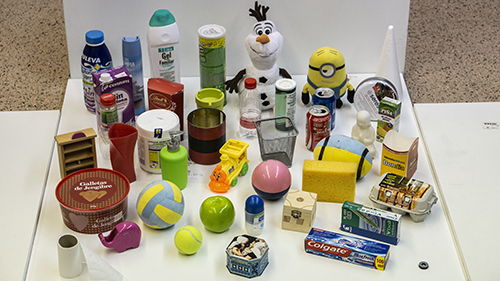
\includegraphics[width=0.95\linewidth]{Figures/Tactile/dataset/trainobjects2-downsampled.jpg}
	\caption{The original training set of $41$ objects.}
	\label{fig:dataset_train}
\end{figure}

\begin{figure}[!htb]
	\centering
	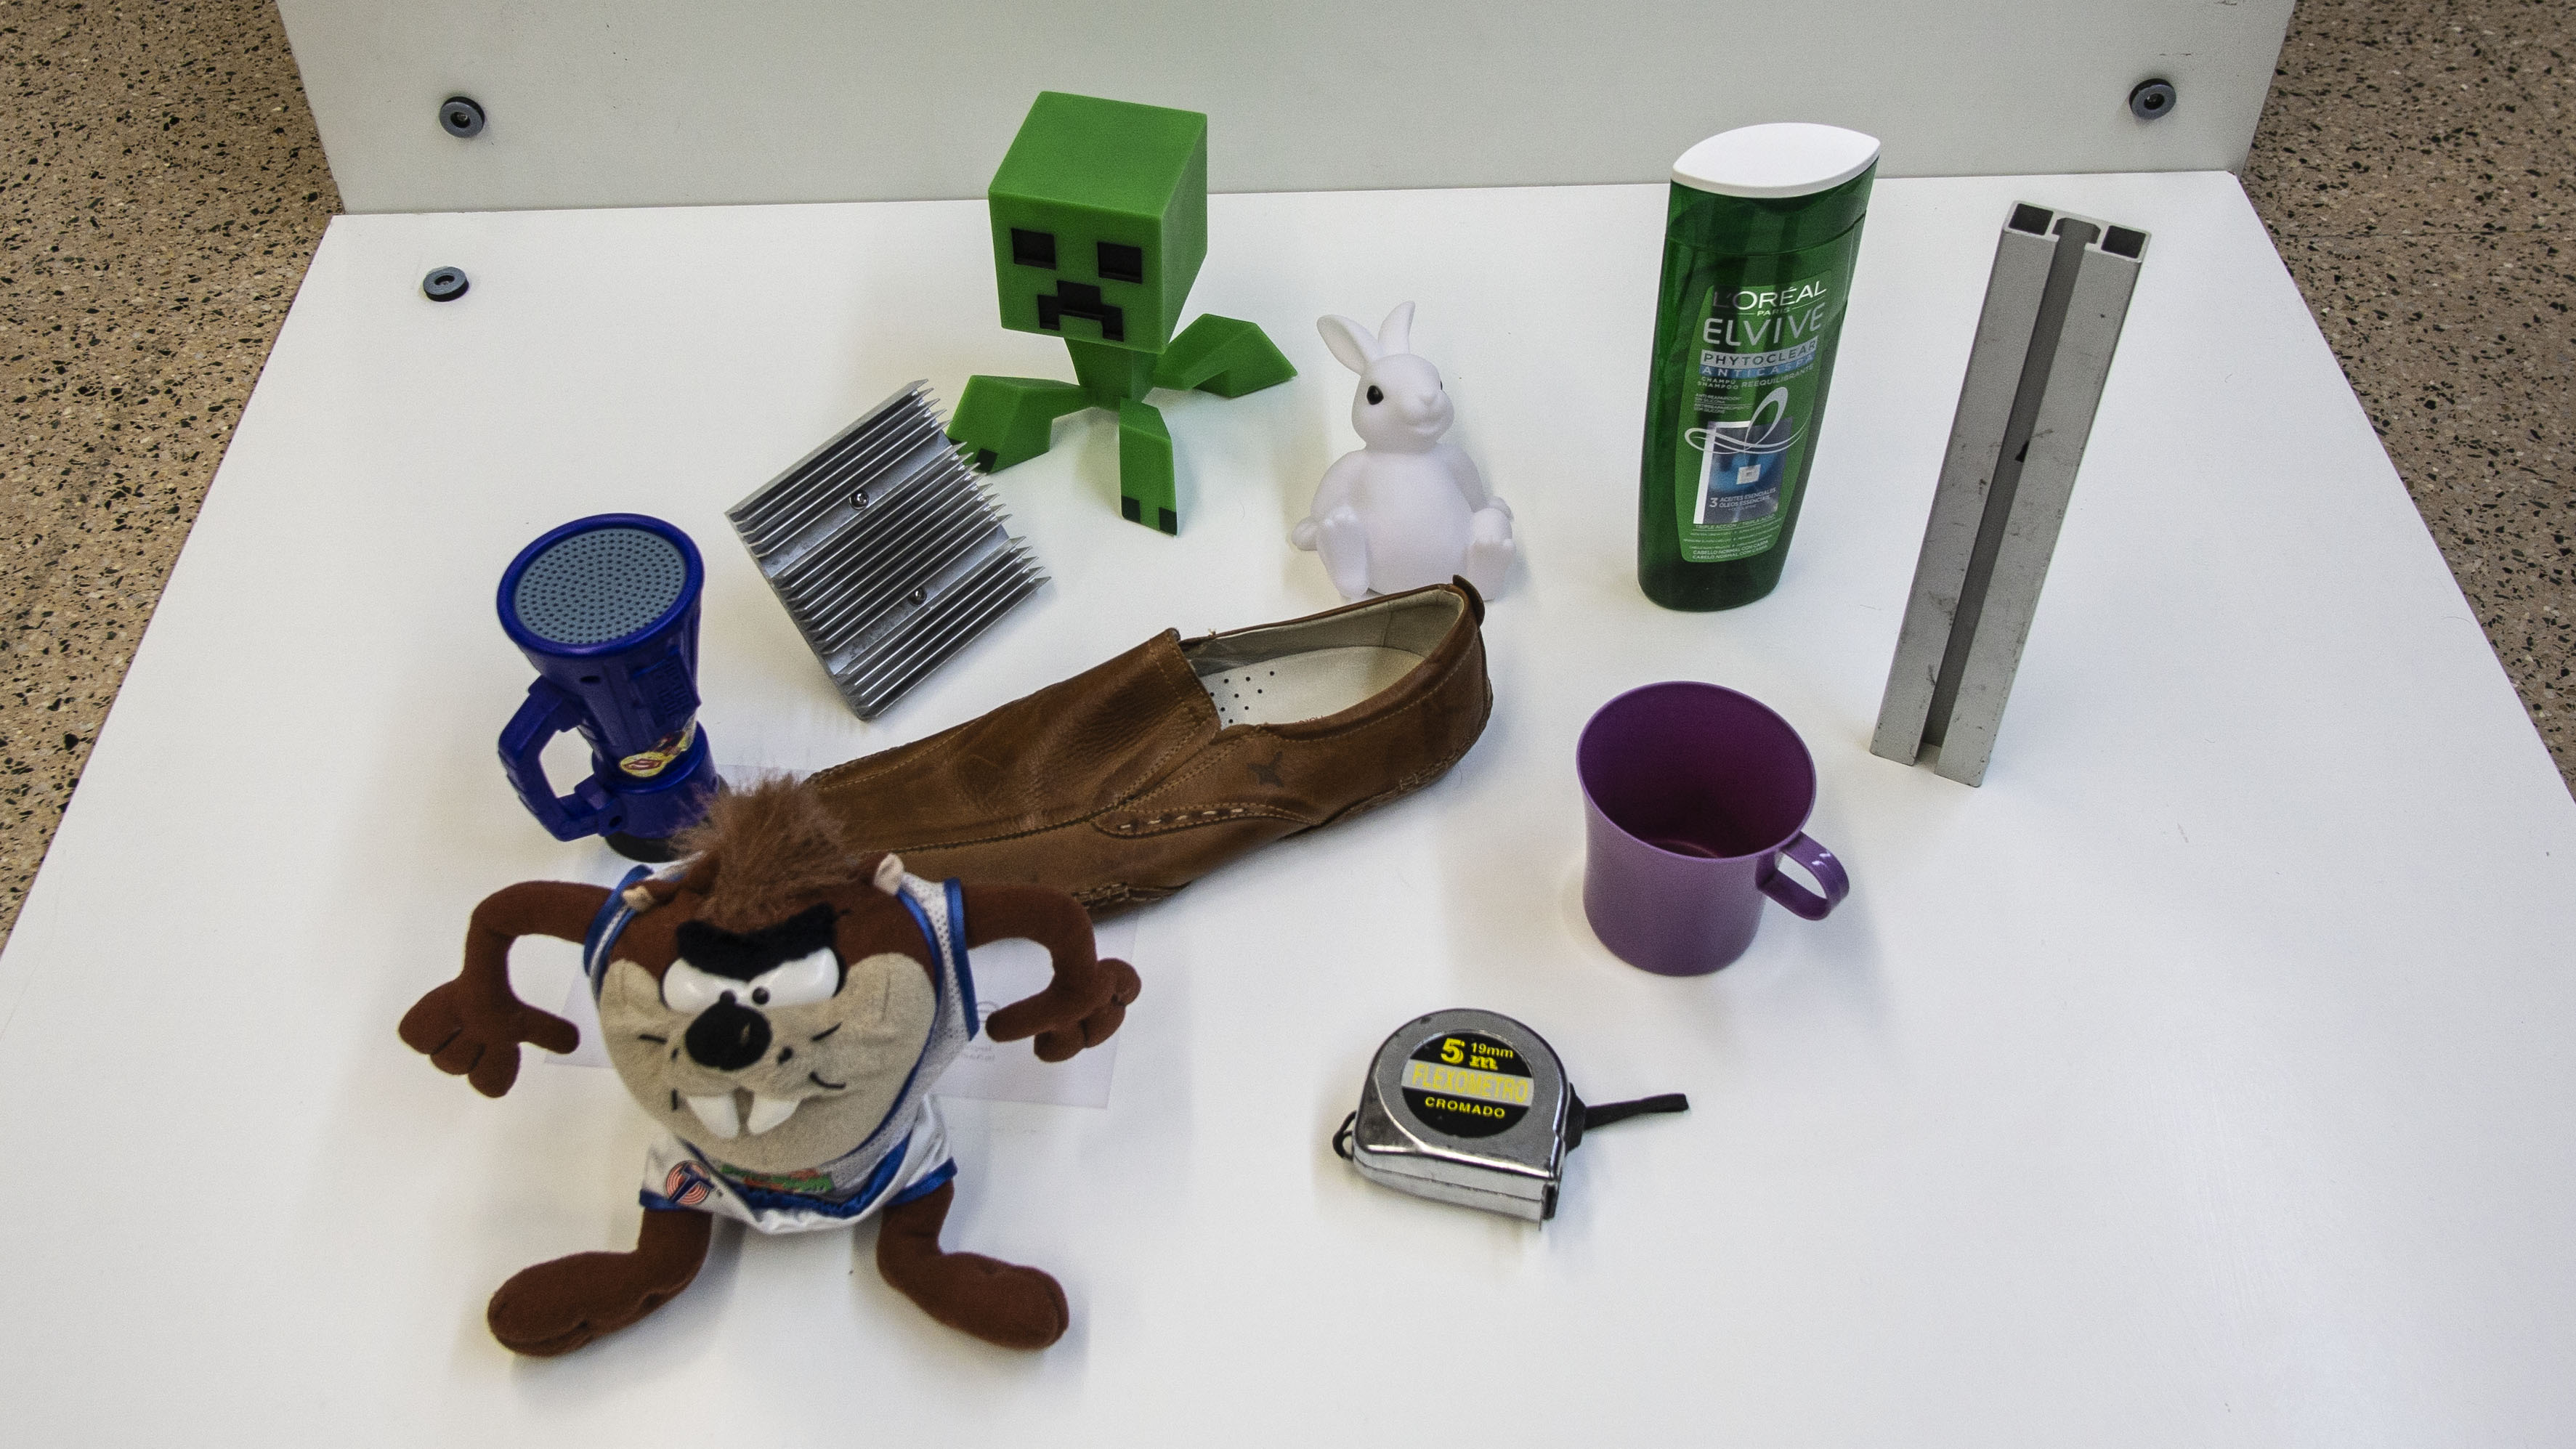
\includegraphics[width=0.95\linewidth]{Figures/Tactile/dataset/testobjects.jpg}
	\caption{The newly captured test set of $10$ objects.}
	\label{fig:dataset_test}
\end{figure}

There are two hand configurations in the original dataset: \textit{palm down} grasps were performed pointing the palm of the hand downwards while \textit{palm side} grasps were recorded pointing it to one side, with the thumb upwards. In this work, we have added a new configuration: \emph{palm 45} which is in between the other two configurations at an angle of $45$ degrees. Figure \ref{fig:dataset_grasps} shows the aforementioned hand configurations.

\begin{figure}[!htb]
	\centering
    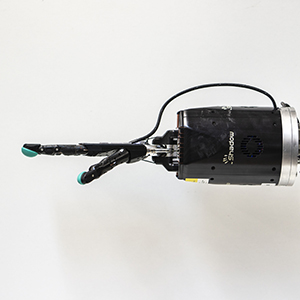
\includegraphics[width=0.32\linewidth]{Figures/Tactile/dataset/palmdown-downsampled}
    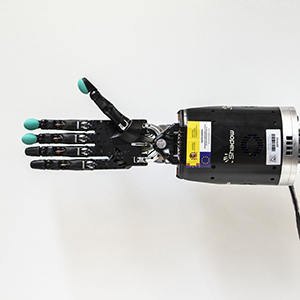
\includegraphics[width=0.32\linewidth]{Figures/Tactile/dataset/palmside-downsampled}
    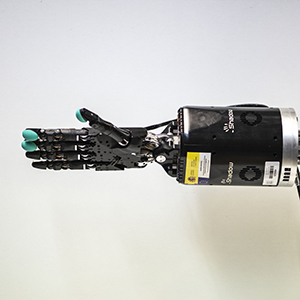
\includegraphics[width=0.32\linewidth]{Figures/Tactile/dataset/palm45-downsampled}\\
    \smallskip
    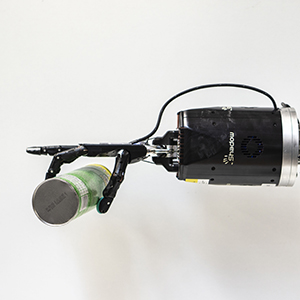
\includegraphics[width=0.32\linewidth]{Figures/Tactile/dataset/palmdown_grasp-downsampled}
    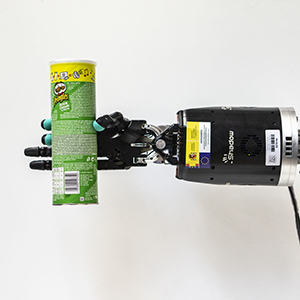
\includegraphics[width=0.32\linewidth]{Figures/Tactile/dataset/palmside_grasp-downsampled}
    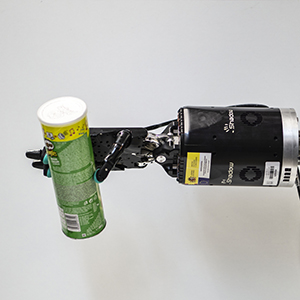
\includegraphics[width=0.32\linewidth]{Figures/Tactile/dataset/palm45_grasp-downsampled}
	\caption{(Top row) Samples of the three hand configurations in the dataset: (from left to right) \emph{palm down}, \emph{palm side}, and \emph{palm 45}. (Bottom row) The same configurations but grasping an object.}
	\label{fig:dataset_grasps}
\end{figure}

Table \ref{table:datasets} provides a quantitative summary of the extended dataset for both splits and all configurations.

\begin{table}[!htb]
	\renewcommand{\arraystretch}{1.3}
	\caption{Summary of the extended BioTac SP dataset which was used in this work to validate our graph-based architecture.}
	\label{table:datasets}
	\centering
	\begin{tabular}{lcccc}
        \hline
        & \multicolumn{2}{c}{\textbf{Training Set}} & \multicolumn{2}{c}{\textbf{Test Set}}\\
        \hline
        \textbf{Configuration} & \textbf{Stable} & \textbf{Slippery}  & \textbf{Stable} & \textbf{Slippery} \\
        \hline
        Palm Down & 667 & 609 & 153 & 163 \\
        Palm Side & 603 & 670 & 157 & 165 \\
        Palm 45 & 1058 & 1075 & 250 & 261 \\
        \hline
        All & 2328 & 2354 & 560 & 589 \\
        \hline           
	\end{tabular}
\end{table}

To the best of our knowledge, there is only one previous work that released a dataset of tactile recordings for the task of grasp stability detection, which is the BiGS dataset \cite{Chebotar2016bigs}. In their work, Chebotar \emph{et al.} recorded 2000 grasps on three standing objects (a cylindrically-shaped box of wipes, a cubically-shaped box of candy and a ball) using a Barret three-fingered hand, which was equipped with three BioTac tactile sensors. Our work extends the BioTac SP
dataset firstly introduced in \cite{Zapata2018}, counting with more than 4000 training grasps and 1000 test grasps with three BioTac SP tactile sensors recorded using 51 objects and various orientations, both for the objects and the hand. The dataset is freely available at GitHub \footnote{\url{https://github.com/3dperceptionlab/biotacsp-stability-set-v2}}.

\subsection{Experimental Setup}

All experiments were run on a computer with an i7-8700 CPU \@ $3.20$ GHz (6 cores / 12 threads) with an Z370 chipset motherboard, 16 GiB DDR4 RAM \@ $2400$ MHz CL15, a Samsung SSD 860 EVO 250 GiB, and an NVIDIA Titan X Maxwell (12 GiB) GPU. Everything was implement in Python $3.6$, PyTorch $0.4.1$, PyTorch Geometric $0.3.1$, CUDA $10.0$ (with driver version $410.73$).

For most experiments, we report accuracy as our main metric to iterate and draw conclusions over training and validation sets. For the test set, we report four different metrics: accuracy, precision, recall, and F1-score (the harmonic mean of precision and recall). To ensure generalization and give an accurate (and statistically correct) estimate of our prediction model performance we employ $k$-fold cross validation with $k=5$. All reported results are the average of $10$ rounds of $5$-fold cross validation. For each cross-validation split, we train our models for $512$ epochs using the ADAM optimizer. The hyperparameters were chosen empirically as follows: $0.01$ learning rate and $5e^{-4}$ weight decay.

The whole source code and dataset for this work can be downloaded from the corresponding GitHub repository\footnote{\url{https://github.com/3dperceptionlab/tactile-gcn}}.

\subsection{Network Depth and Width}

In these experiments, we investigate the impact of network depth (convolution layers) and width (amount of features per layer). To that end, we have tested ten different models ranging from one to ten \emph{GCNConv} layers with increasing number of features ($8$, $16$, $32$, $48$, $64$). ReLU activations were used after each convolutional layer. Two fully connected layers were also placed at the end of the network (with $128$ and $2$ output features respectively) to produce the classification
result. We made use of the manually defined graph connections ($k=0$). Figure \ref{fig:experiments_width_depth} shows the results of this set of experiments.

\begin{figure}[!htb]
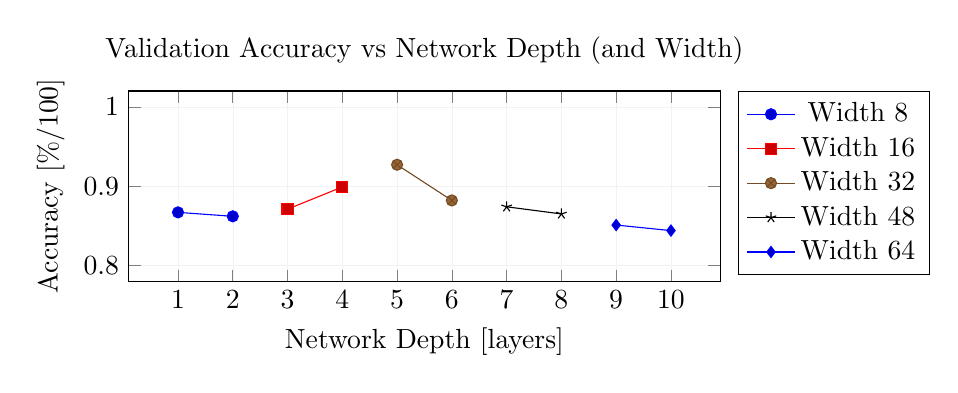
\begin{tikzpicture}
\begin{axis}[
    width=0.75\linewidth,
    height=4cm,
    title={Validation Accuracy vs Network Depth (and Width)},
    xlabel={Network Depth [layers]},
    ylabel={Accuracy [\%/100]},
    xmin=1, xmax=10,
    ymin=0.8, ymax=1,
    xtick={1, 2, 3, 4, 5, 6, 7, 8, 9, 10},
    ytick={0.0, 0.1, 0.2, 0.3, 0.4, 0.5, 0.6, 0.7, 0.8, 0.9, 1.0},
    legend pos=outer north east,
    grid style={line width=.1pt, draw=gray!10},
    ymajorgrids=true,
    xmajorgrids=true,
    enlargelimits=true,
]

  \addplot
    coordinates {
      (1, 0.867)(2, 0.862)
    };
  \addplot
    coordinates {
      (3, 0.871)(4, 0.899)
    };
  \addplot
    coordinates {
      (5, 0.927)(6, 0.882)
    };
  \addplot
    coordinates {
      (7, 0.874)(8, 0.865)
    };
  \addplot
    coordinates {
      (9, 0.851)(10, 0.844)
    };
  \legend{Width 8, Width 16, Width 32, Width 48, Width 64}
\end{axis}
\end{tikzpicture}
  \caption{Results of network depth and width study.}
  \label{fig:experiments_width_depth}
\end{figure}

As we can observe, there is a dependency on both width and depth. Shallow networks tend to perform better than their deep counterparts. However, we can find a sweet spot on the architecture with $5$ layers and $32$ features ($8-8-16-16-32$). Shallower networks are not able to fully capture our problem while deeper ones tend to overfit our training data. Consequently, we will proceed with that network.

\subsection{Graph Connectivity}

For the connectivity experiments we took the previous best network and investigated the effect of graph connectivity. We experimented with manually specified edges ($k=0$) and the \ac{k-NN} strategy with $k = [1, 23]$. As shown in Figure \ref{fig:experiments_connectivity}, the performance of the network degraded as the connectivity of the graph increased in each experiment. Using the \ac{k-NN} strategy, smaller $k$ values achieved greater performance in terms of validation accuracy. However,
none of them improved the performance ($92.7\%$) yielded by the network trained with the graph created using the manual connectivity ($k = 0$).

In the manually created graph there are electrodes connected by an edge to just one other electrode, some others are connected up to four neighbors and the electrode in the center (24th electrode) is connected to six other points. As a result, there are different degrees of connectivity within the graph that could have given some insight to the network about the importance of each node in order to better learn the problem.

\begin{figure}[!htb]
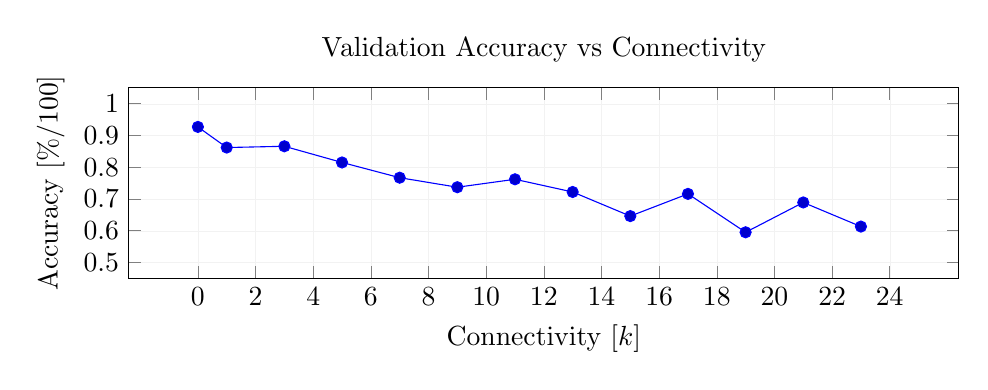
\begin{tikzpicture}
\begin{axis}[
    width=\linewidth,
    height=4cm,
    title={Validation Accuracy vs Connectivity},
    xlabel={Connectivity [$k$]},
    ylabel={Accuracy [\%/100]},
    xmin=0, xmax=24,
    ymin=0.50, ymax=1,
    xtick={0, 2, 4, 6, 8, 10, 12, 14, 16, 18, 20, 22, 24},
    ytick={0.0, 0.1, 0.2, 0.3, 0.4, 0.5, 0.6, 0.7, 0.8, 0.9, 1.0},
    grid style={line width=.1pt, draw=gray!10},
    ymajorgrids=true,
    xmajorgrids=true,
    enlargelimits=true,
]

  \addplot
    coordinates {
      (0, 0.927)(1, 0.862)(3, 0.866)(5, 0.815)(7, 0.767)(9, 0.737)(11, 0.762)(13, 0.722)(15, 0.646)(17, 0.716)(19, 0.595)(21, 0.689)(23, 0.613)
    };
\end{axis}
\end{tikzpicture}
  \caption{Performance of the network according to the connectivity of the graph.}
  \label{fig:experiments_connectivity}
\end{figure}

\subsection{Generalization Tests}

In order to prove the generalization capabilities of our system, we trained our best network ($8-8-16-16-32$ with $k=0$) with our whole training set and evaluated it on the various test sets (palm down, palm side and palm 45). All results are reported in Table \ref{table:generalization_tests}.

\begin{table}[!htb]
  \centering
    \caption{Results of generalization experiments on the testing splits.}
    \label{table:generalization_tests}
    \begin{tabular}{r|cccc}
        \hline
        \textbf{Test Set} & \textbf{Accuracy} & \textbf{Precision} & \textbf{Recall} & \textbf{F1}\\
        \hline
        Down & 0.741 & 0.741 & 0.751 & 0.745\\
        45 & 0.774 & 0.774 & 0.783 & 0.778\\
        Side & 0.751 & 0.785 & 0.709 & 0.745\\
        \hline
    \end{tabular}
\end{table}

There is a significant drop in accuracy when dealing with completely unknown objects. Recall that the test set consists of new objects with different geometries and stiffness levels so they are substantially different from the training set. Taking all of this into account, and despite the difficulty of the testing set, we can expect gains from applying regularization and augmentation strategies to increase performance on data whose distribution is not that similar to the training set.

\section{Conclusion}
\label{cha:tactile:sec:conclusion}

Tactile sensors provide useful information for robotic manipulation tasks like predicting grasp stability. Prior works in the literature tend to compute hand-engineered features that are later used for training a machine learning model. A recent trend process them as images, so deep learning techniques like \acsp{CNN} can calculate relevant characteristics that lets the system distinguish a slippery grasp from a stable one. Inspired by this methodology, we propose in this work a novel approach to tactile data interpretation: we build a graph with the sensor's taxels because this structure keeps more accurately the spatial distribution and the local connectivity of these sensing points. The goodness of these properties and the tactile graph for grasp stability prediction were tested in experimentation.

We used three BioTac SP tactile sensors mounted in the tip of the index, middle and thumb of a Shadow Dexterous hand. In order to predict grasp stability using these graph representations of the tactile sensors, we trained a \ac{GCN} with a custom dataset which was captured with more than 50 objects and 3 hand orientations. The robustness of the proposed system was checked by testing the system with novel orientations and objects. In average, the \ac{GCN} yielded a 92.7\% validation accuracy on the prediction of grasp stability with novel objects or orientations.

\subsection{Limitations and Future Works}
\label{cha:tactile:sec:conclusion:subsec:limitations}

Given the obtained results, graph representations of tactile readings can be successfully used for learning the task of grasp stability prediction. Nevertheless, there are some drawbacks linked to their used. The first limitation of this proposal is the problem of defining the graph connectivity. We had to find a way of defining the location of the taxels as well as their connections in order to define the graph. In the case of using the tactile readings directly, none of this is necessary.

Moreover, \ac{GCN} showed to be data hungry models for learning. In a previous work \cite{Zapata2018}, the authors obtained higher validation rates ($94.2\%$) with fewer data samples for training a \ac{CNN}. For this work, it was necessary to capture more data in order to achieve similar accuracy rates in training. Furthermore, generalization to radically new objects has still a lot of room for improvement by leveraging techniques such as L2 regularization, dropout, or data augmentation
itself.

As a future work, we also plan to decouple the currently unified \ac{GCN} for the three fingers so that each graph is processed by a different network path. Furthermore, we plan to model the noise of each individual taxel and augment each sample on the fly by adding random noise following each taxel's distribution. At last, we plan to extend the architecture to predict grasp stability over temporal sequences by fusing the \ac{GCN} model with \ac{LSTM} networks.